\section{Results}
\label{sec:results}

\subsection{Claim 1}

\paragraph{Tracking Attention Logits}
To reproduce Claim 1, we monitor the \textbf{maximum attention logits} in the first Transformer layer. This choice is motivated their empirical observations showing that early layers exhibit the largest logits and are the first to diverge.
We compare two configurations: with \texttt{qk-layernorm} and without \texttt{qk-layernorm}, and for each setting we run the experiments with learning rate $\eta \in \{0.1,\ 0.03,\ 0.01,\ 0.003\}$
\begin{figure}[H]
    \centering
    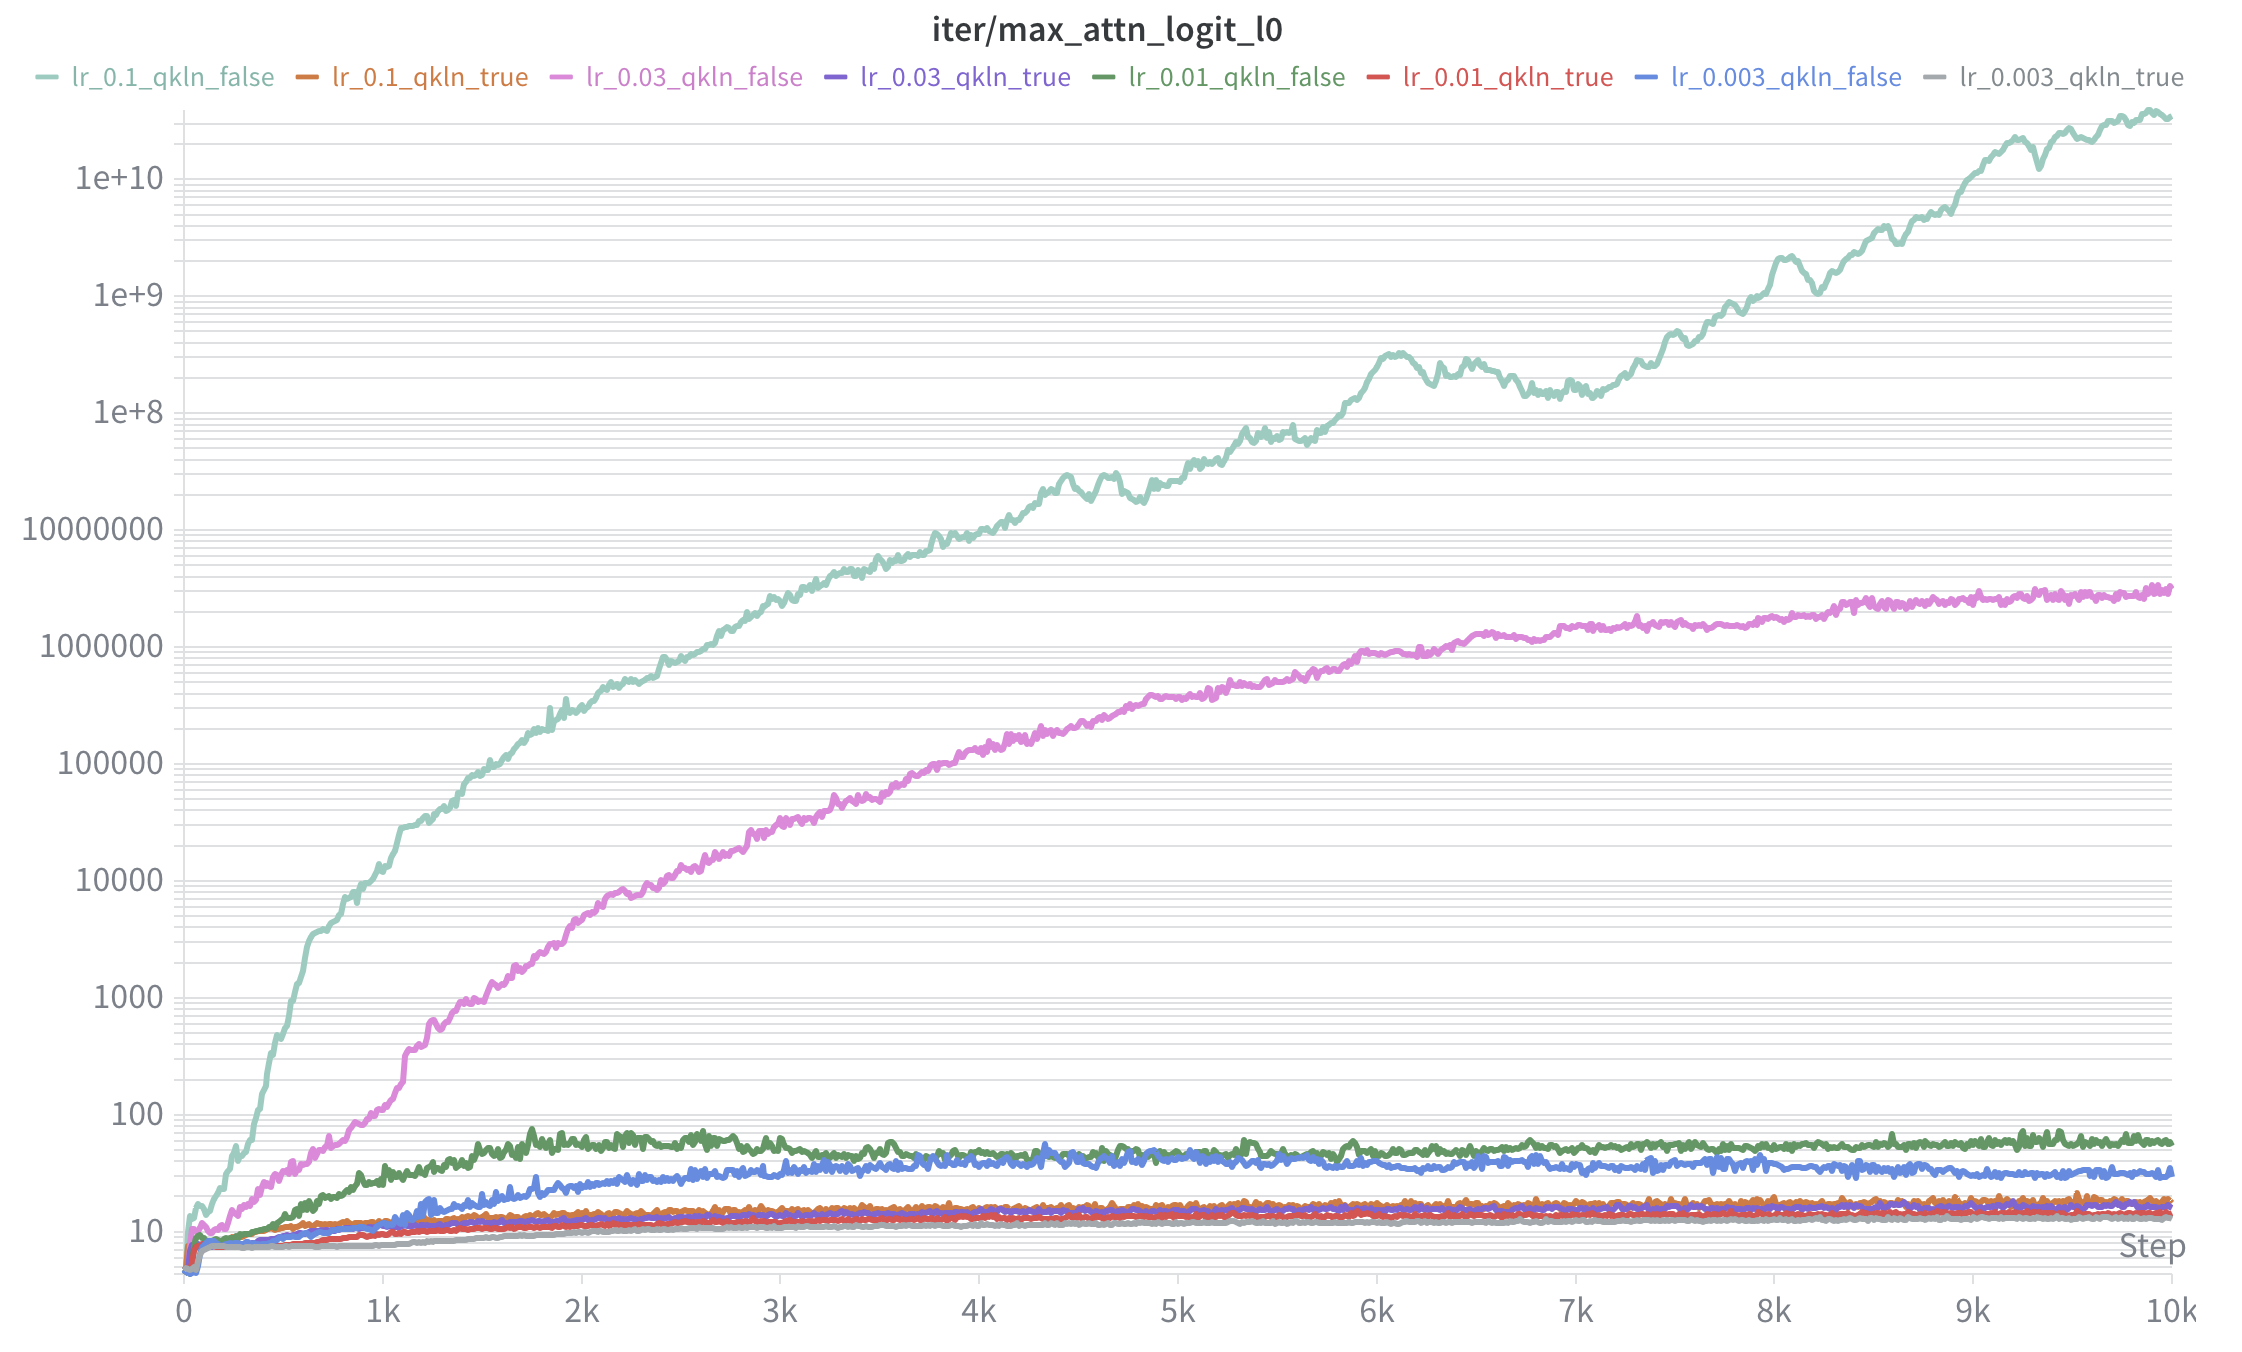
\includegraphics[width=0.7\linewidth]{figures/C1_max_attn_logits.png}
    \caption{Evolution of the maximum attention logits in the first layer. Divergence occurs at high learning rates when qk-layernorm is not used.}
\end{figure}
We observe that attention logits diverge when: $\eta \geq 0.03 \quad \text{and qk-layernorm is disabled}$. And this behavior is consistent with their findings. We then report the following learning rate sensitivy : \textbf{0.025} with qk-layernorm and \textbf{1.37} without, and  (unfortunately it is not a curve depending, only for a given parameters size, here $\approx$50M), which follows their results. 



\paragraph{Origin of the Instability: Norm Explosion} To confirm the origin of this divergence, we track the mean norms of queries and keys, and observe that the norms of $Q$ and $K$ increase rapidly, reproducing the results proposed in appendix of the paper. 
\begin{figure}[H]
\centering
\begin{subfigure}{0.48\linewidth}
    \centering
    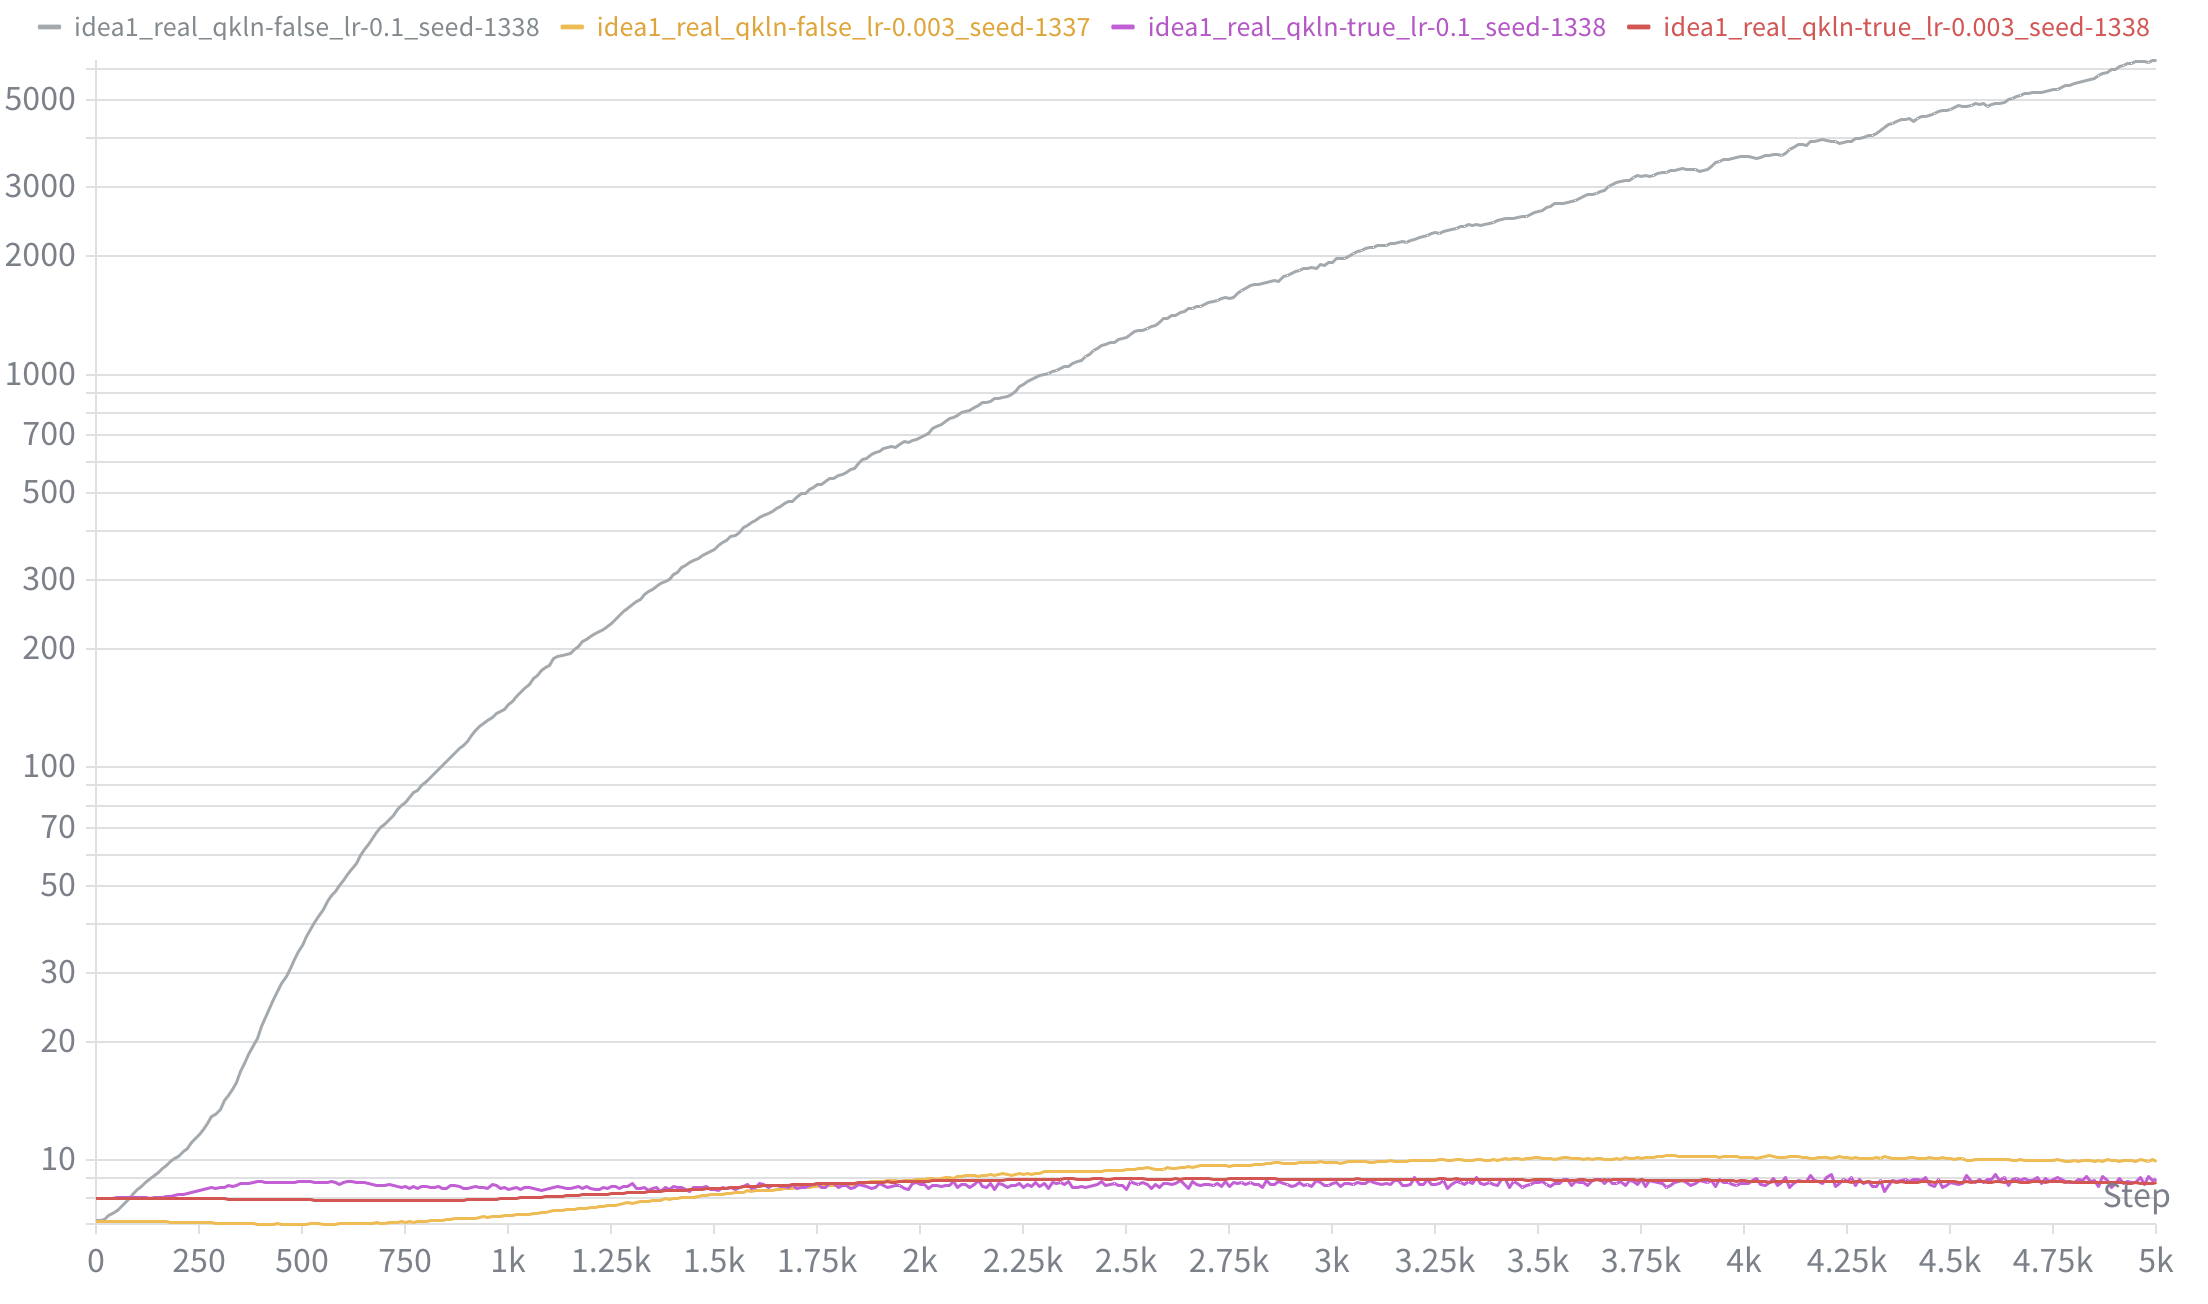
\includegraphics[width=\linewidth]{figures/C1_qnorm.png}
    \caption{Mean norm of $Q$}
\end{subfigure}
\hfill
\begin{subfigure}{0.48\linewidth}
    \centering
    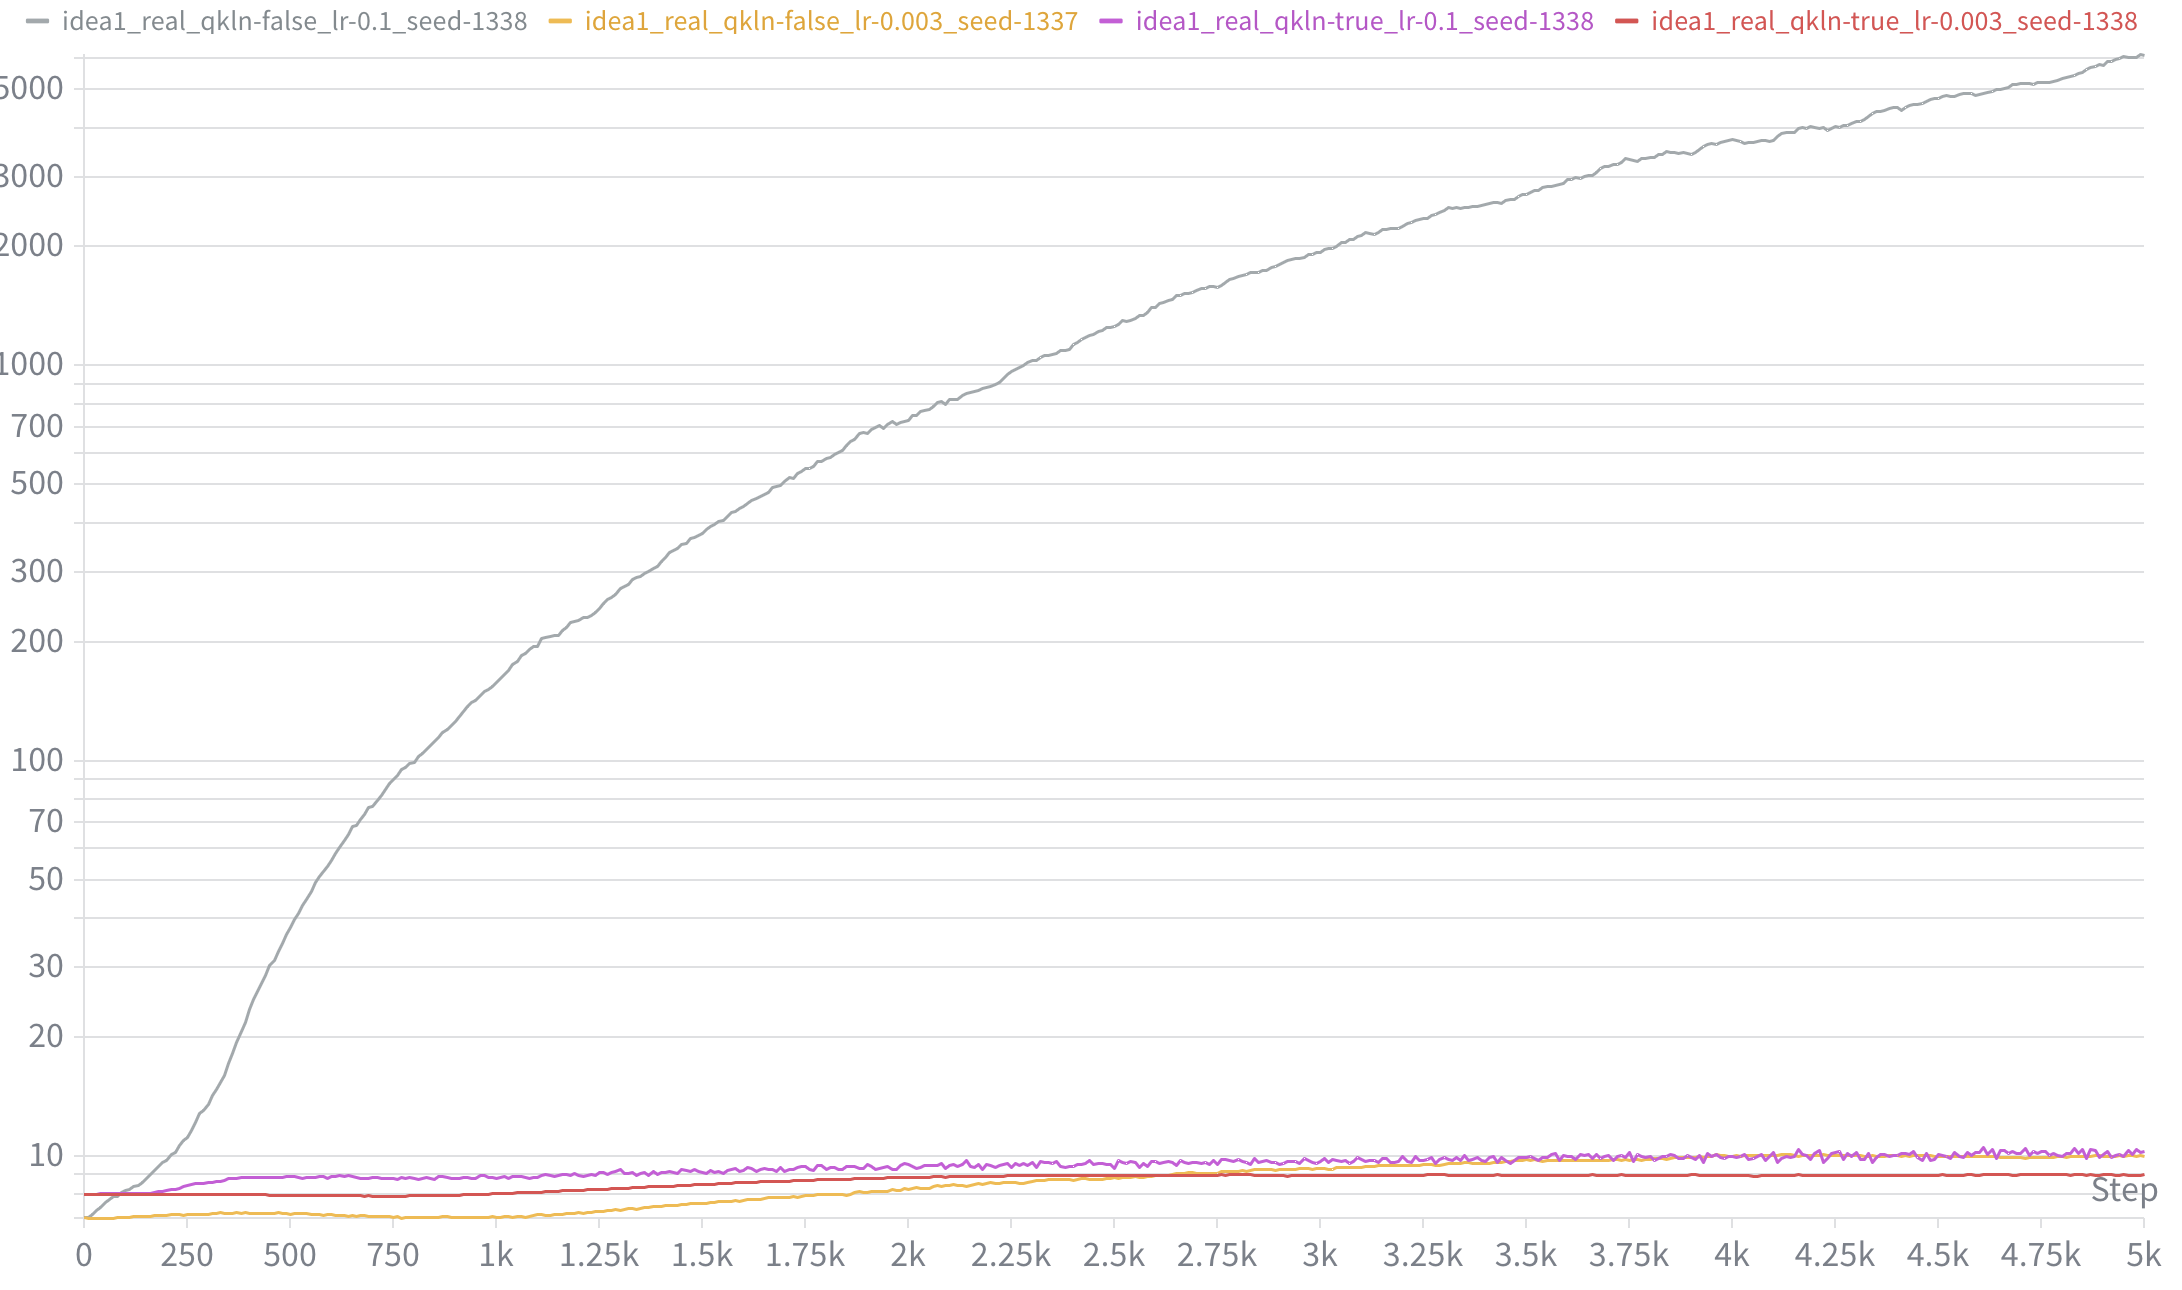
\includegraphics[width=\linewidth]{figures/C1_knorm.png}
    \caption{Mean norm of $K$}
\end{subfigure}
\caption{Evolution of query and key norms in the first attention layer.}
\end{figure}


\paragraph{Optimizer vs Data: Robustness Analysis}
In theory, for gradient descent, to avoid divergence, one requires with $\eta$ the learning rate : 
\[
\eta < \frac{2}{\lambda_{\max}(H)} \text{  and where $H$ is the Hessian of the loss: } H_{ij} = \frac{\partial^2 \mathcal{L}}{\partial \theta_i \partial \theta_j}
\]
This quantity is too large to compute in practice, but can be approximated. Moreover, $H$ depends on the parameters, but also on the training process and therefore on the data $\mathcal{D}$ : $H = H(\theta_{\text{step}}, \mathcal{D})$
where the dynamic is included in $\theta_{\text{step}}$ (as noted by the authors, the curvature varies during training). The \textit{data-driven} aspect can be interpreted as defining the global loss landscape, while the \textit{optimization-driven} aspect determines where we are located in this landscape and how we evolve within it.

The original work suggests that this instability is optimizer-driven rather than data-dependent. We validate this hypothesis by comparing different dataset constructions. A dataset is said to be IID (independent and identically distributed) if: $x_1, x_2, \dots, x_n \sim \mathcal{D}$ where all samples are independent and drawn from the same distribution. In practice, this removes any sequential or structural dependencies. A shuffled dataset consists of the same samples but randomly permuted. Unlike IID data, local dependencies may still exist, but global ordering is destroyed. 

\begin{figure}[H]
\centering
\begin{subfigure}{0.48\linewidth}
    \centering
    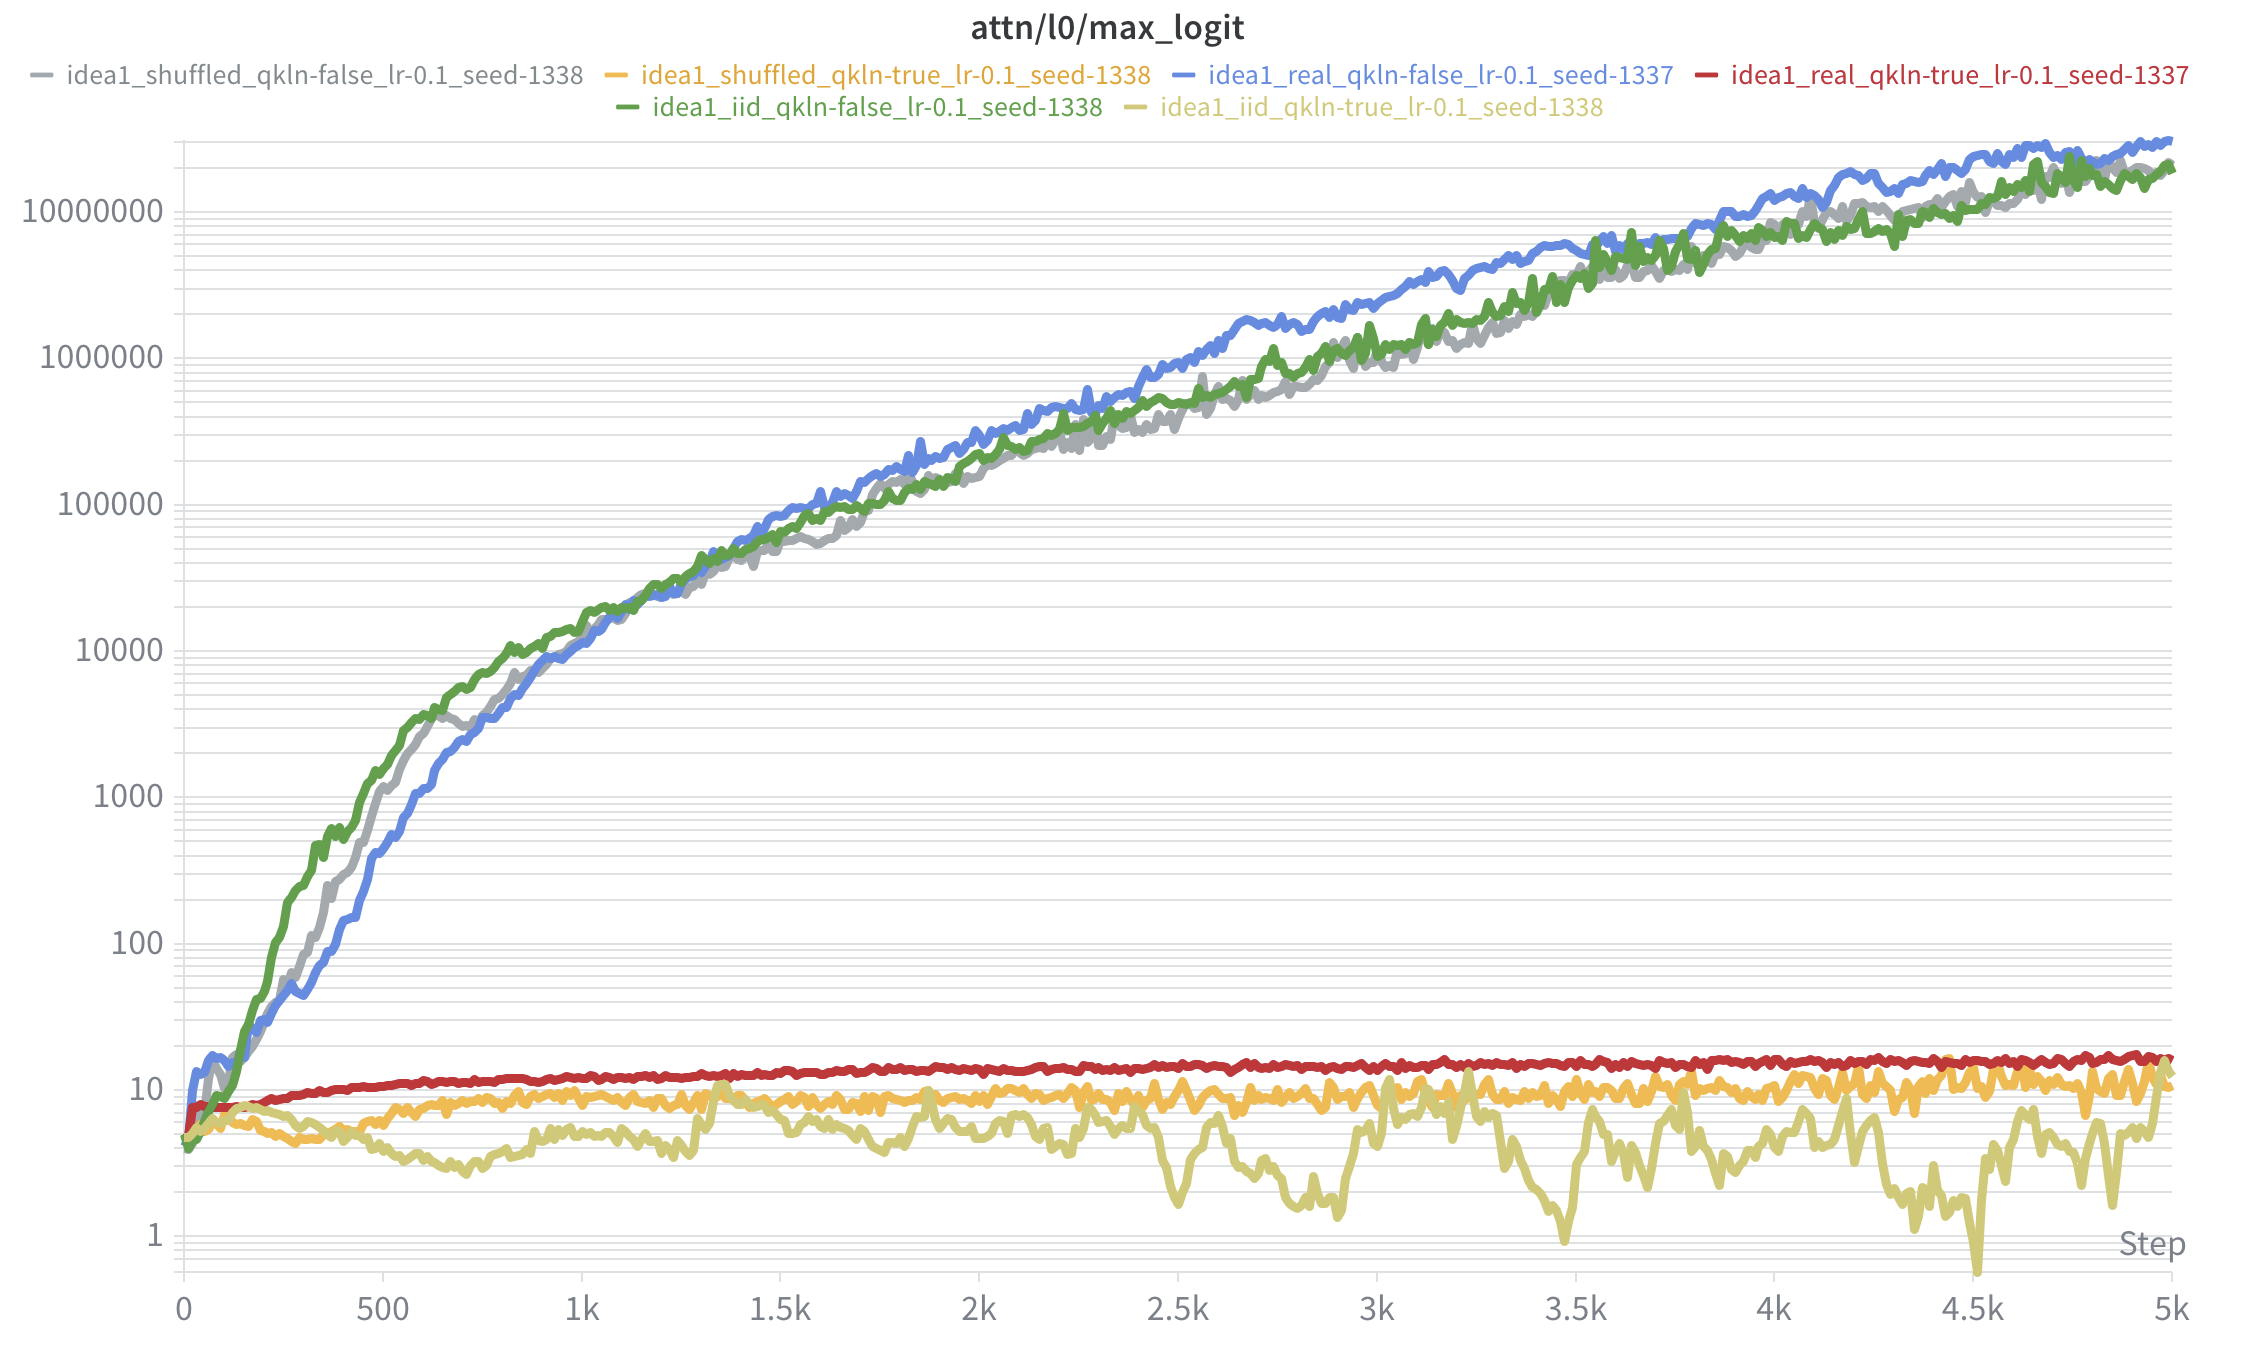
\includegraphics[width=\linewidth]{figures/C1_multiple_data.png}
    \caption{Maximum attention logits}
\end{subfigure}
\hfill
\begin{subfigure}{0.48\linewidth}
    \centering
    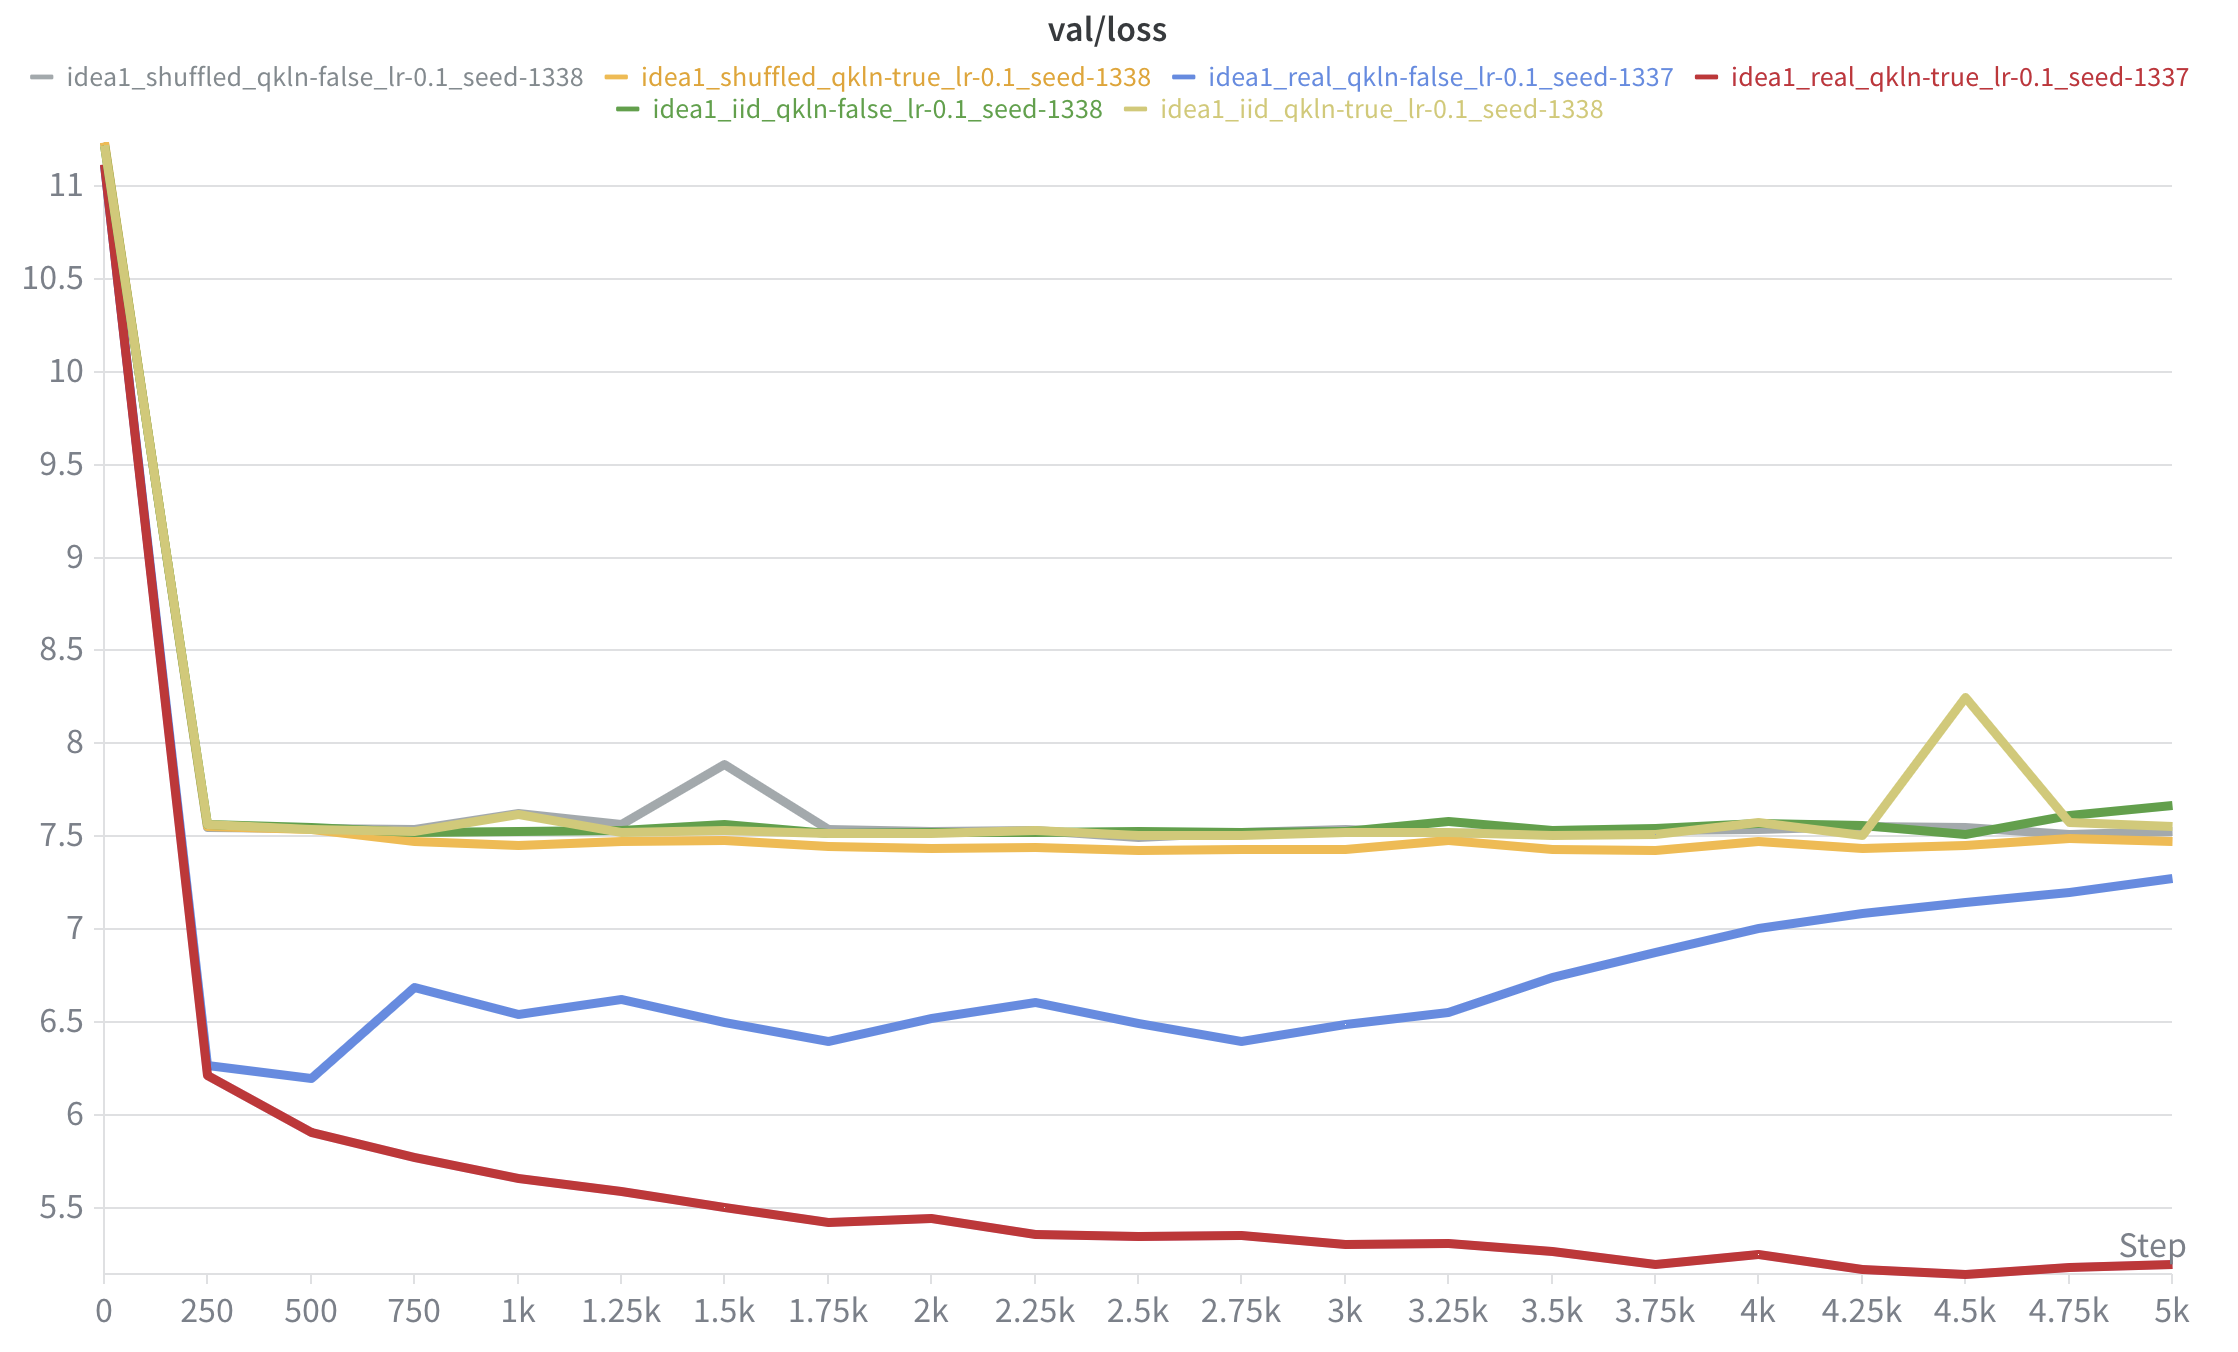
\includegraphics[width=\linewidth]{figures/C1_losses_datasets.png}
    \caption{Validation loss}
\end{subfigure}
\caption{Comparison across standard, shuffled, and IID datasets. Note that for iid and shuffled it is higher as the model can only overfit the training data without learning to generalize.}
\end{figure}
As we observe that logit divergence occurs in all settings, our experiments confirm that instabilities are more driven by the dynamics:
\[
\text{stability} \sim \frac{\eta}{\lambda_{\max}(H(\theta_{\text{step}}, \mathcal{D}))}
\approx \frac{\eta}{\lambda_{\max}(H(\theta_{\text{step}}))}.
\]




\subsection{Claim 2}

Our reproduction of Claim~2 was ultimately unsuccessful.
While the paper reports a clear output-logit divergence when weight decay is
removed, we did not observe the same phenomenon reliably in our small-scale
setting.
Across the runs we carried out, the mean output logit either remained
comparatively well-behaved, or training became unstable in a more global and
less interpretable way before any clean divergence pattern emerged.

To make the instability easier to trigger, we deliberately explored more
aggressive training settings than our default setup.
In particular, we disabled gradient clipping, increased the learning rate,
removed learning-rate warmup, and disabled learning-rate decay.
These changes were intended to stress the optimisation dynamics and reproduce
the failure mode described in the paper more quickly.
However, this did not lead to a convincing confirmation of the claim.

Instead, we observed two broad outcomes.
In some runs, training remained stable enough that the output logit mean did
not exhibit the expected runaway behaviour, even in the no-weight-decay
configuration.
In other runs, optimisation became unstable more abruptly, with large training
pathologies that made the behaviour difficult to attribute specifically to the
output-logit mechanism discussed by~\citet{wortsman2023smallscale}.
As a result, our experiments do not provide clear evidence that removing weight
decay alone causes the output logit mean to explode in our setting, nor do they
allow us to cleanly isolate the stabilising effect of z-loss.

We nevertheless report representative figures from these runs.
They illustrate the main outcome of our reproduction attempt: depending on the
configuration, we observed either no clear divergence in the output logit mean
or severe overall optimisation instability, but not the clean qualitative
pattern described in the original paper.

\begin{figure}[H]
    \centering

    % -------- Row 1: Stable --------
    \begin{subfigure}{0.48\textwidth}
        \centering
        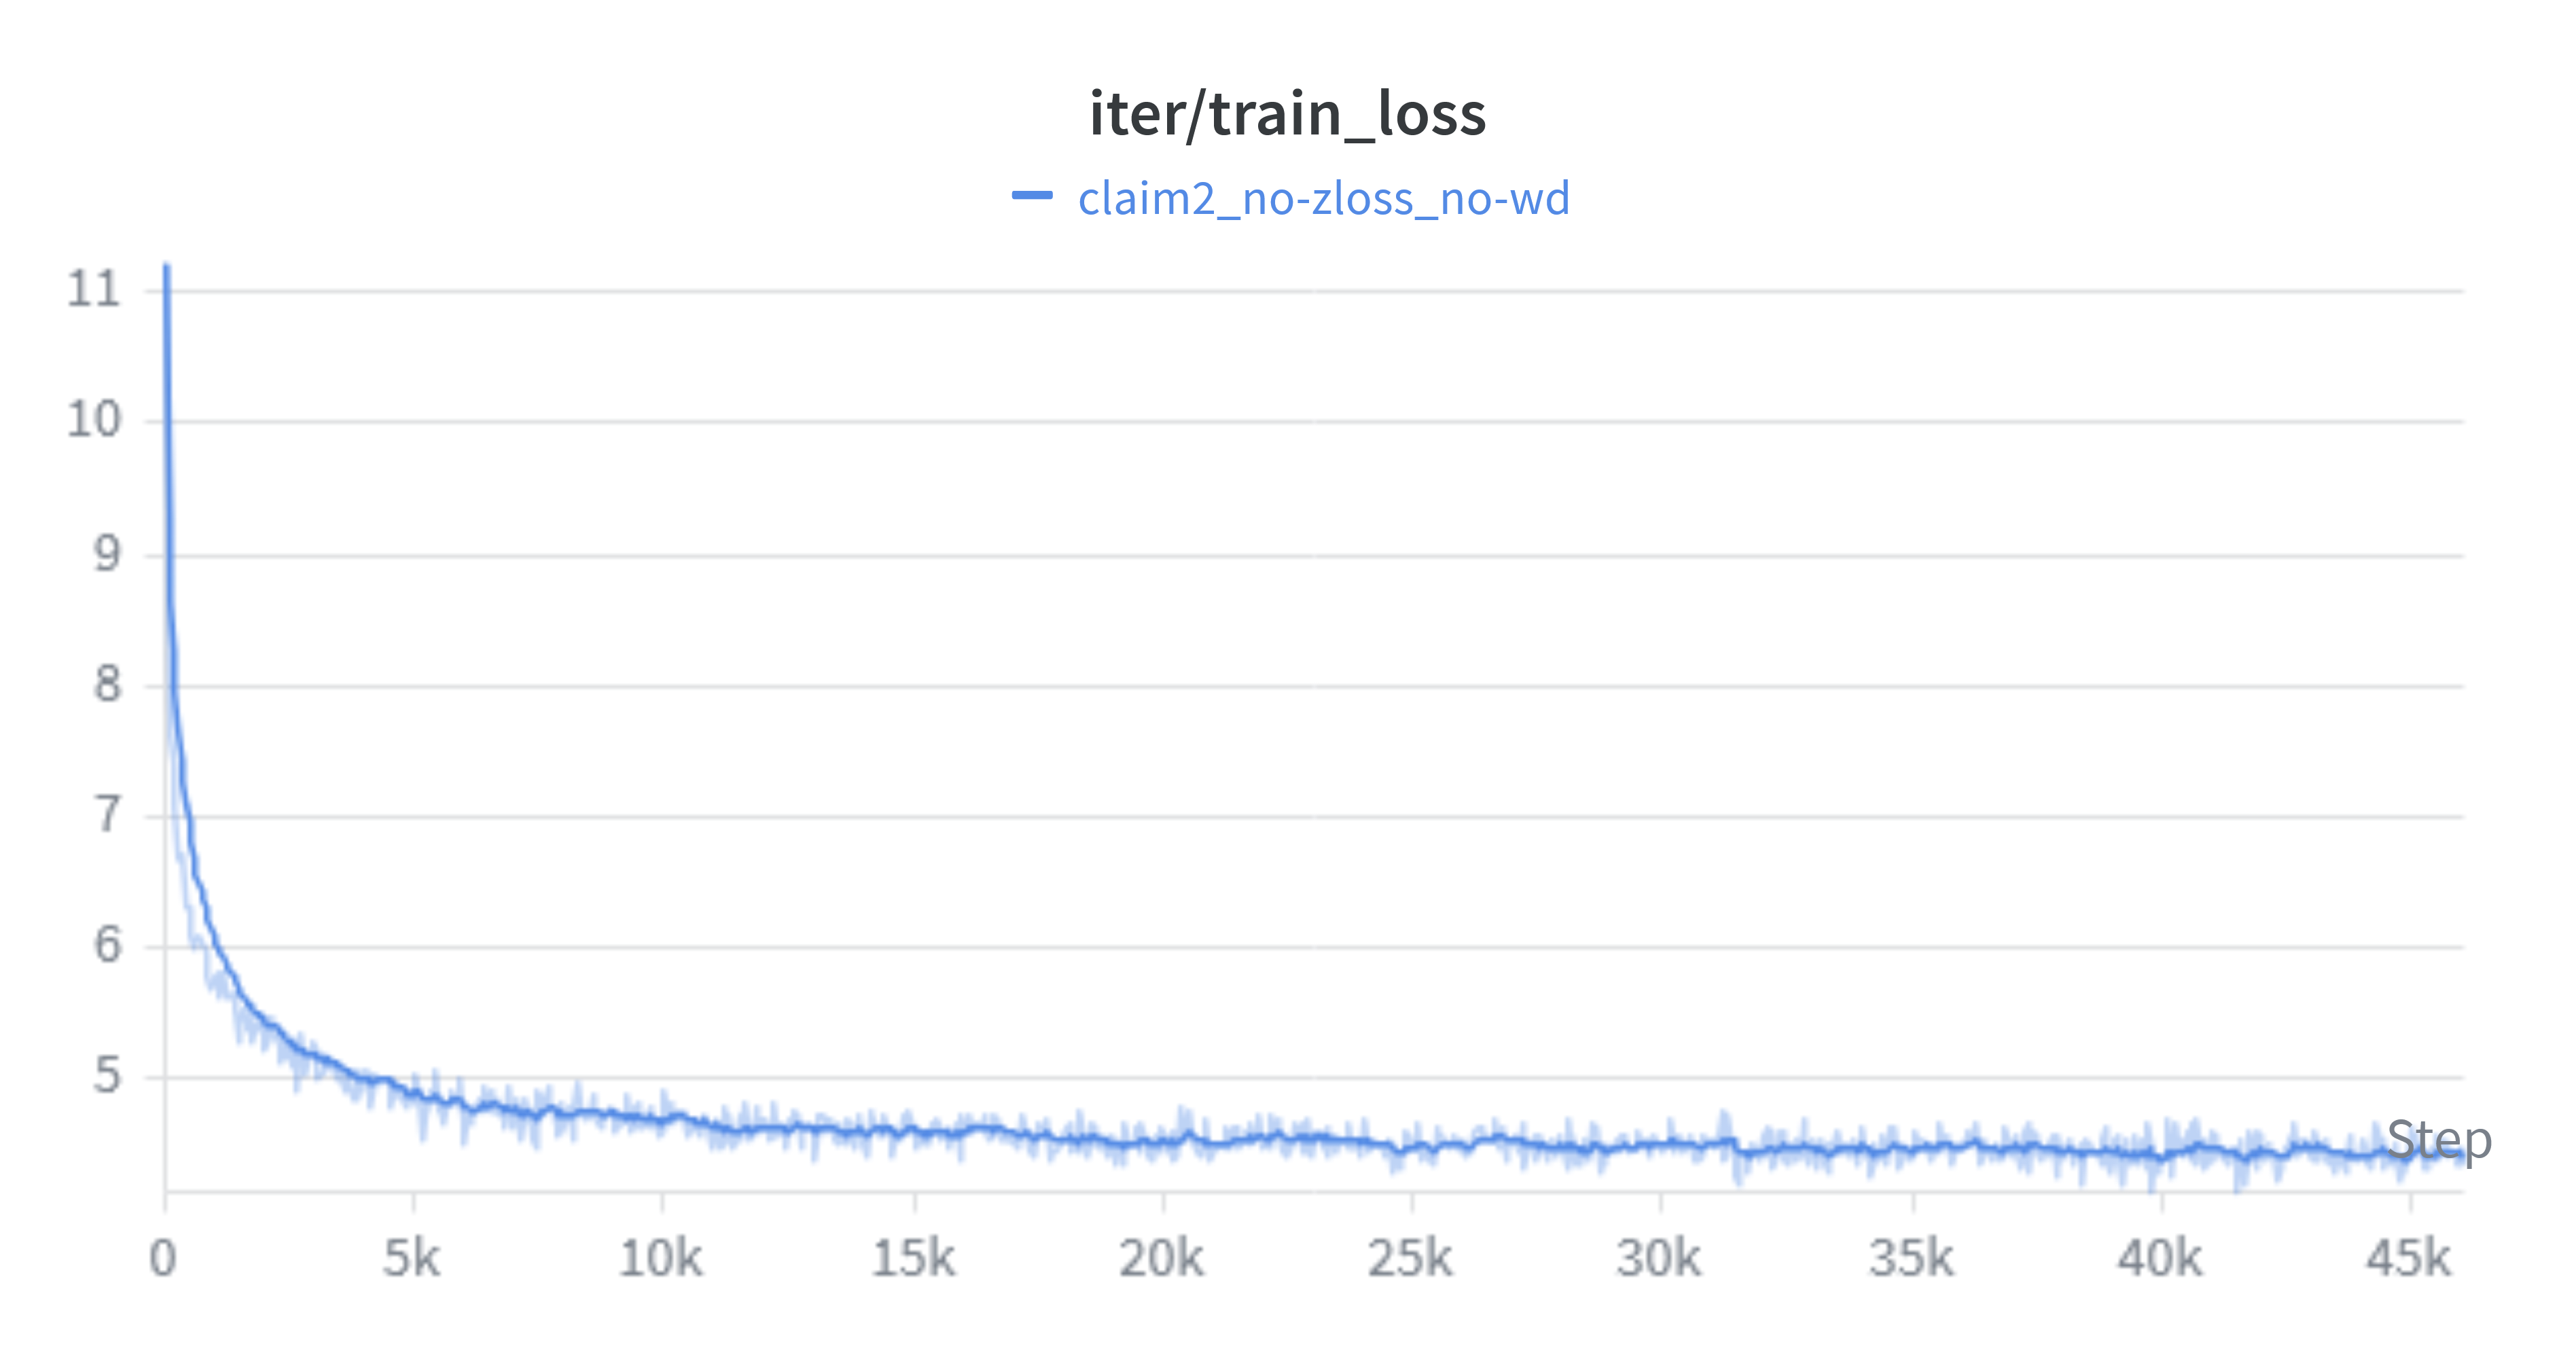
\includegraphics[width=\linewidth]{figures/C2_train_loss_stable.png}
        \caption{Stable — train loss}
    \end{subfigure}
    \hfill
    \begin{subfigure}{0.48\textwidth}
        \centering
        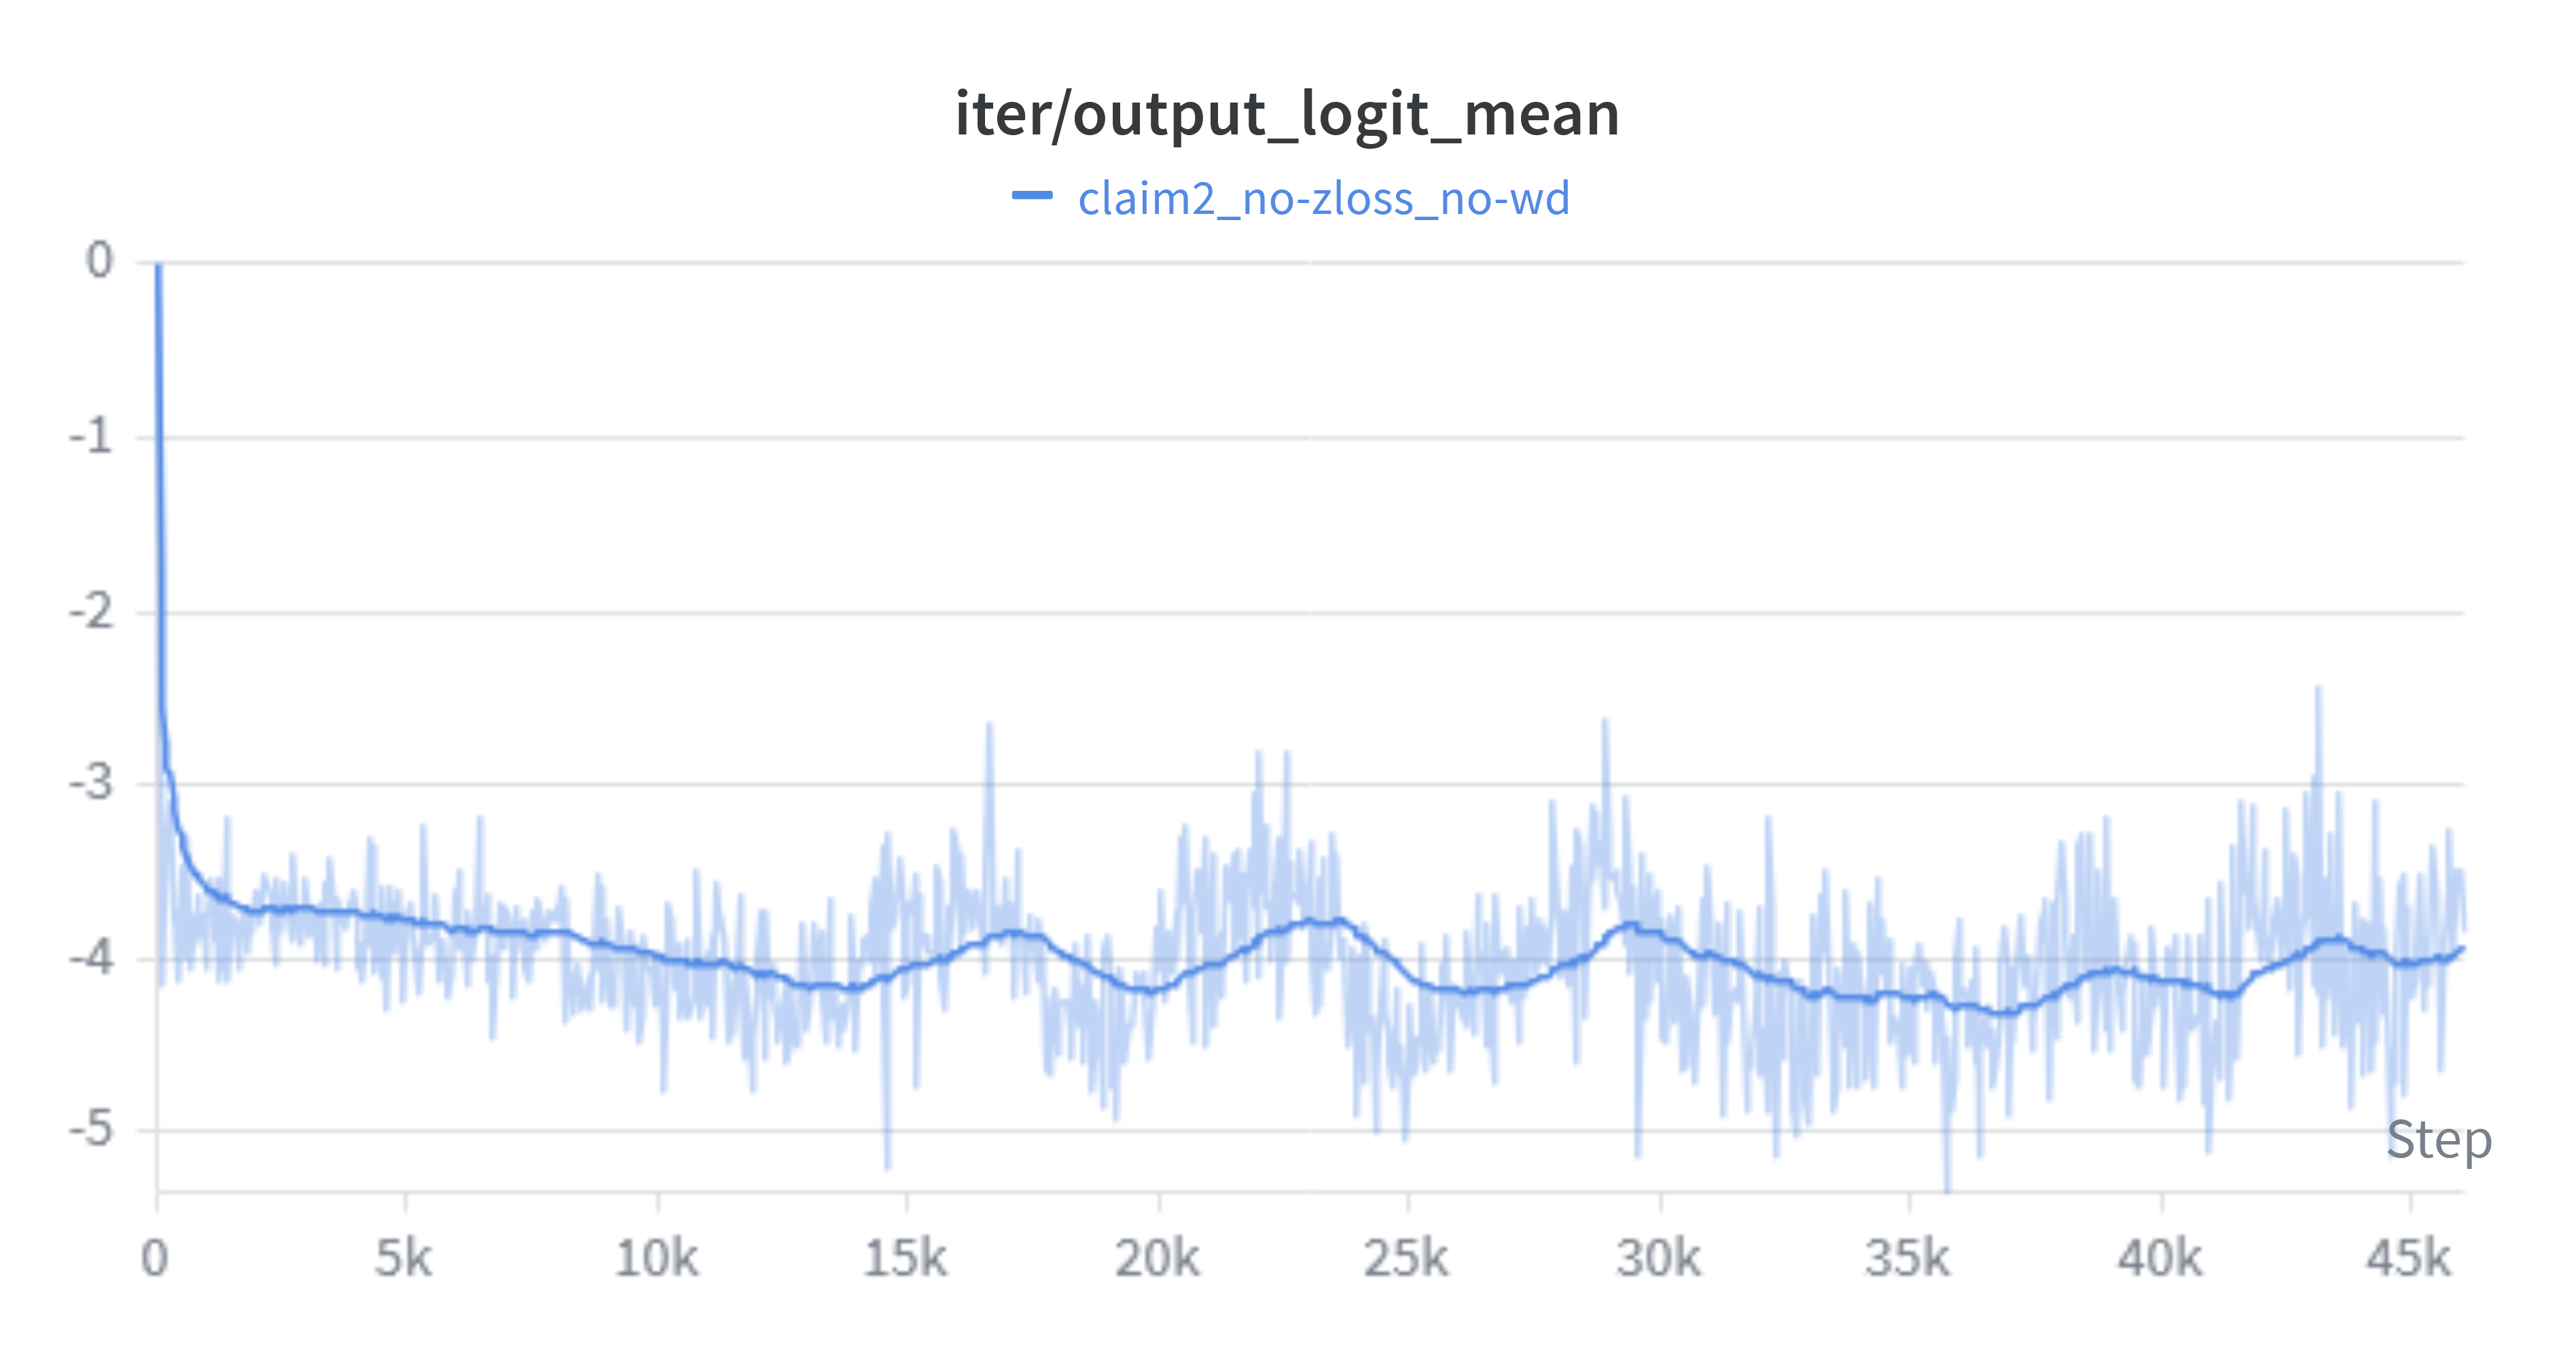
\includegraphics[width=\linewidth]{figures/C2_logit_mean_stable.png}
        \caption{Stable — logit mean}
    \end{subfigure}

    \vspace{0.5em}

    % -------- Row 2: OK stable --------
    \begin{subfigure}{0.48\textwidth}
        \centering
        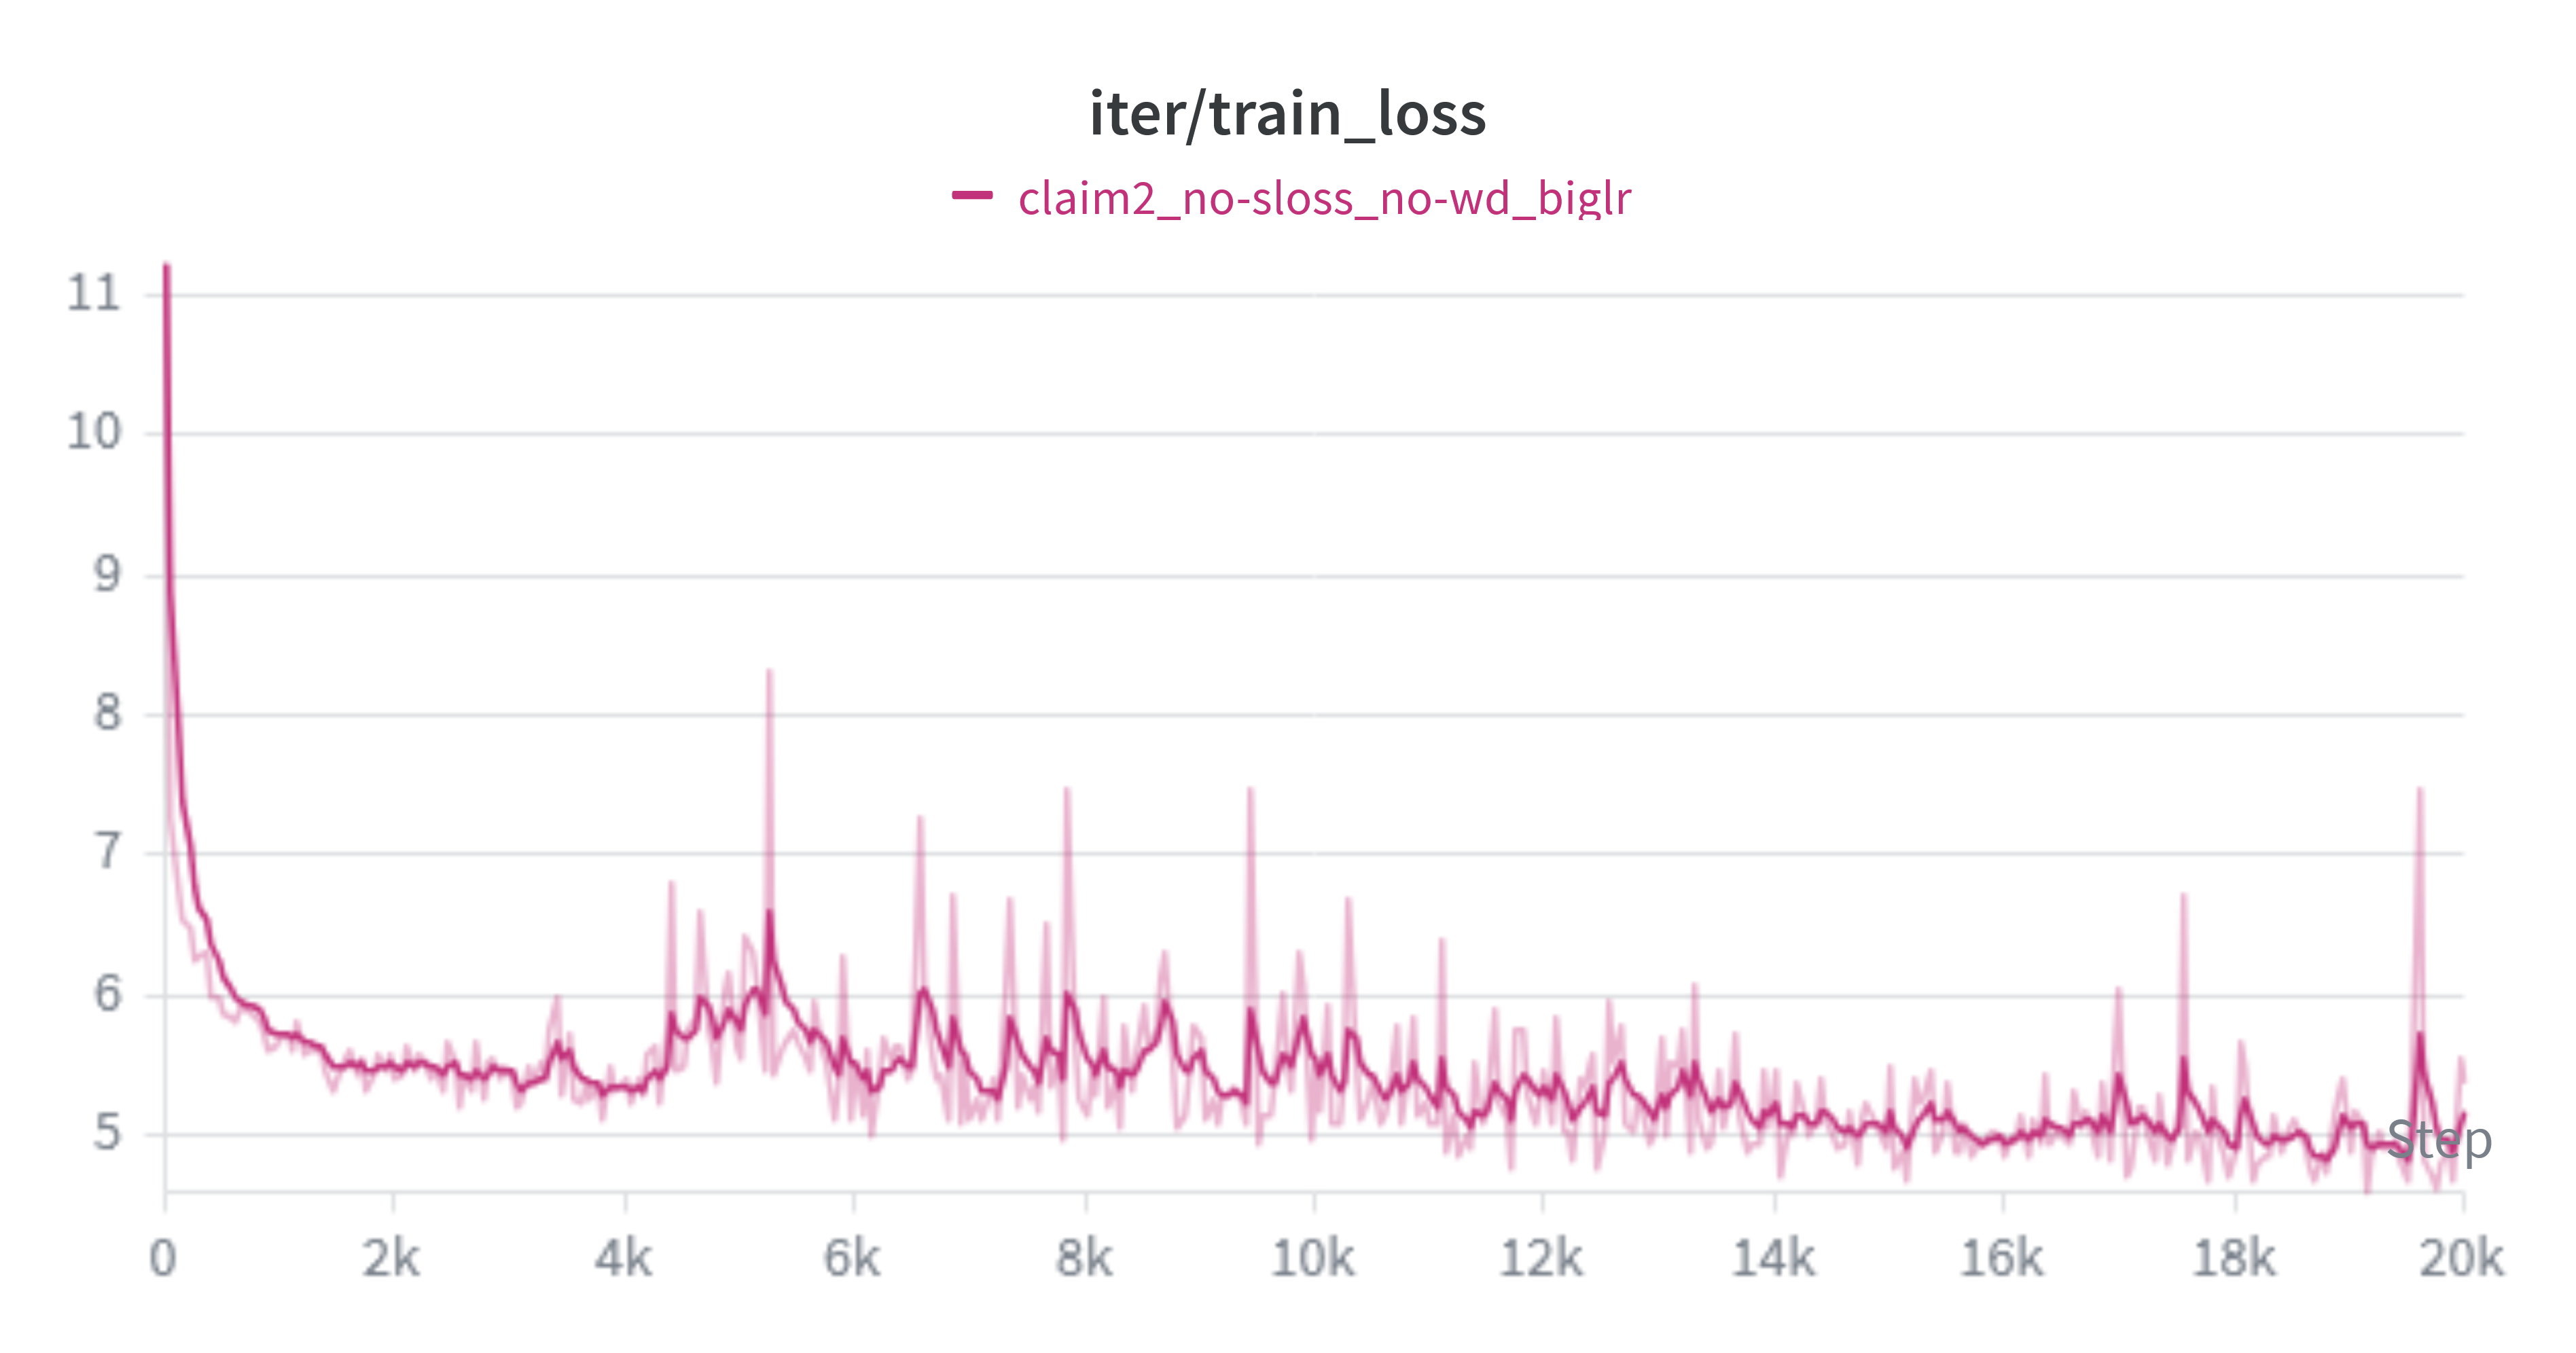
\includegraphics[width=\linewidth]{figures/C2_train_loss_mehstable.png}
        \caption{Moderately stable — train loss}
    \end{subfigure}
    \hfill
    \begin{subfigure}{0.48\textwidth}
        \centering
        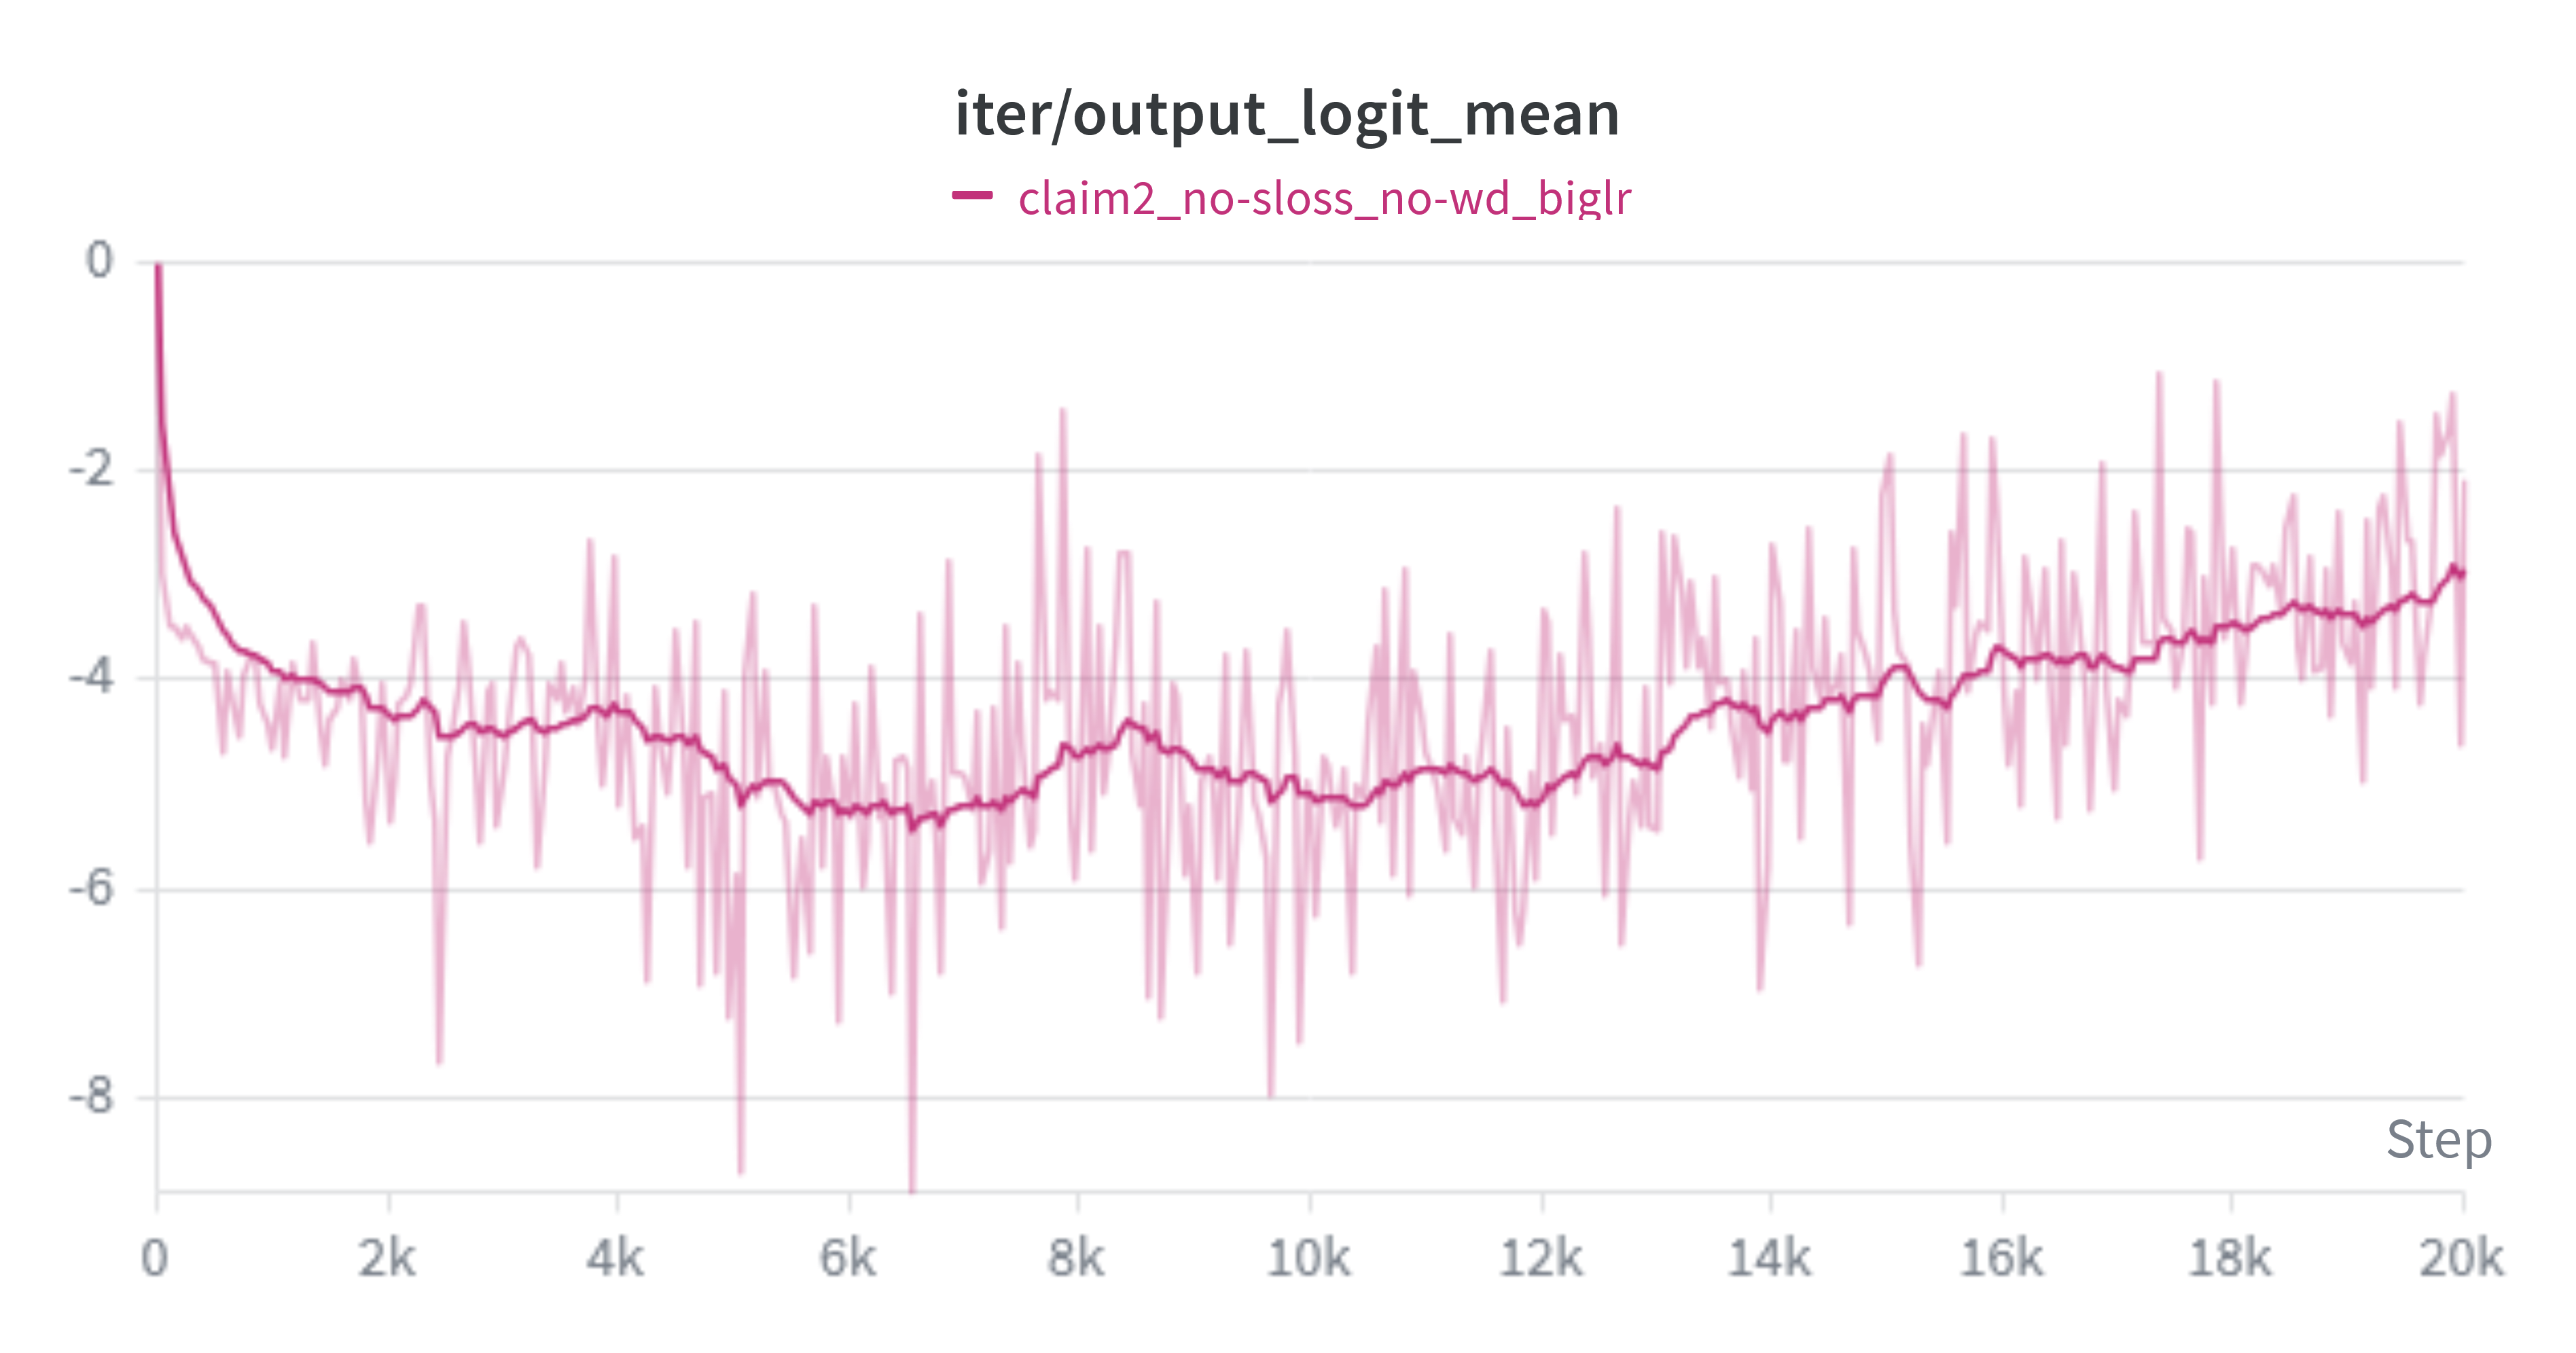
\includegraphics[width=\linewidth]{figures/C2_mean_meh_stable.png}
        \caption{Moderately stable — logit mean}
    \end{subfigure}

    \vspace{0.5em}

    % -------- Row 3: Unstable --------
    \begin{subfigure}{0.48\textwidth}
        \centering
        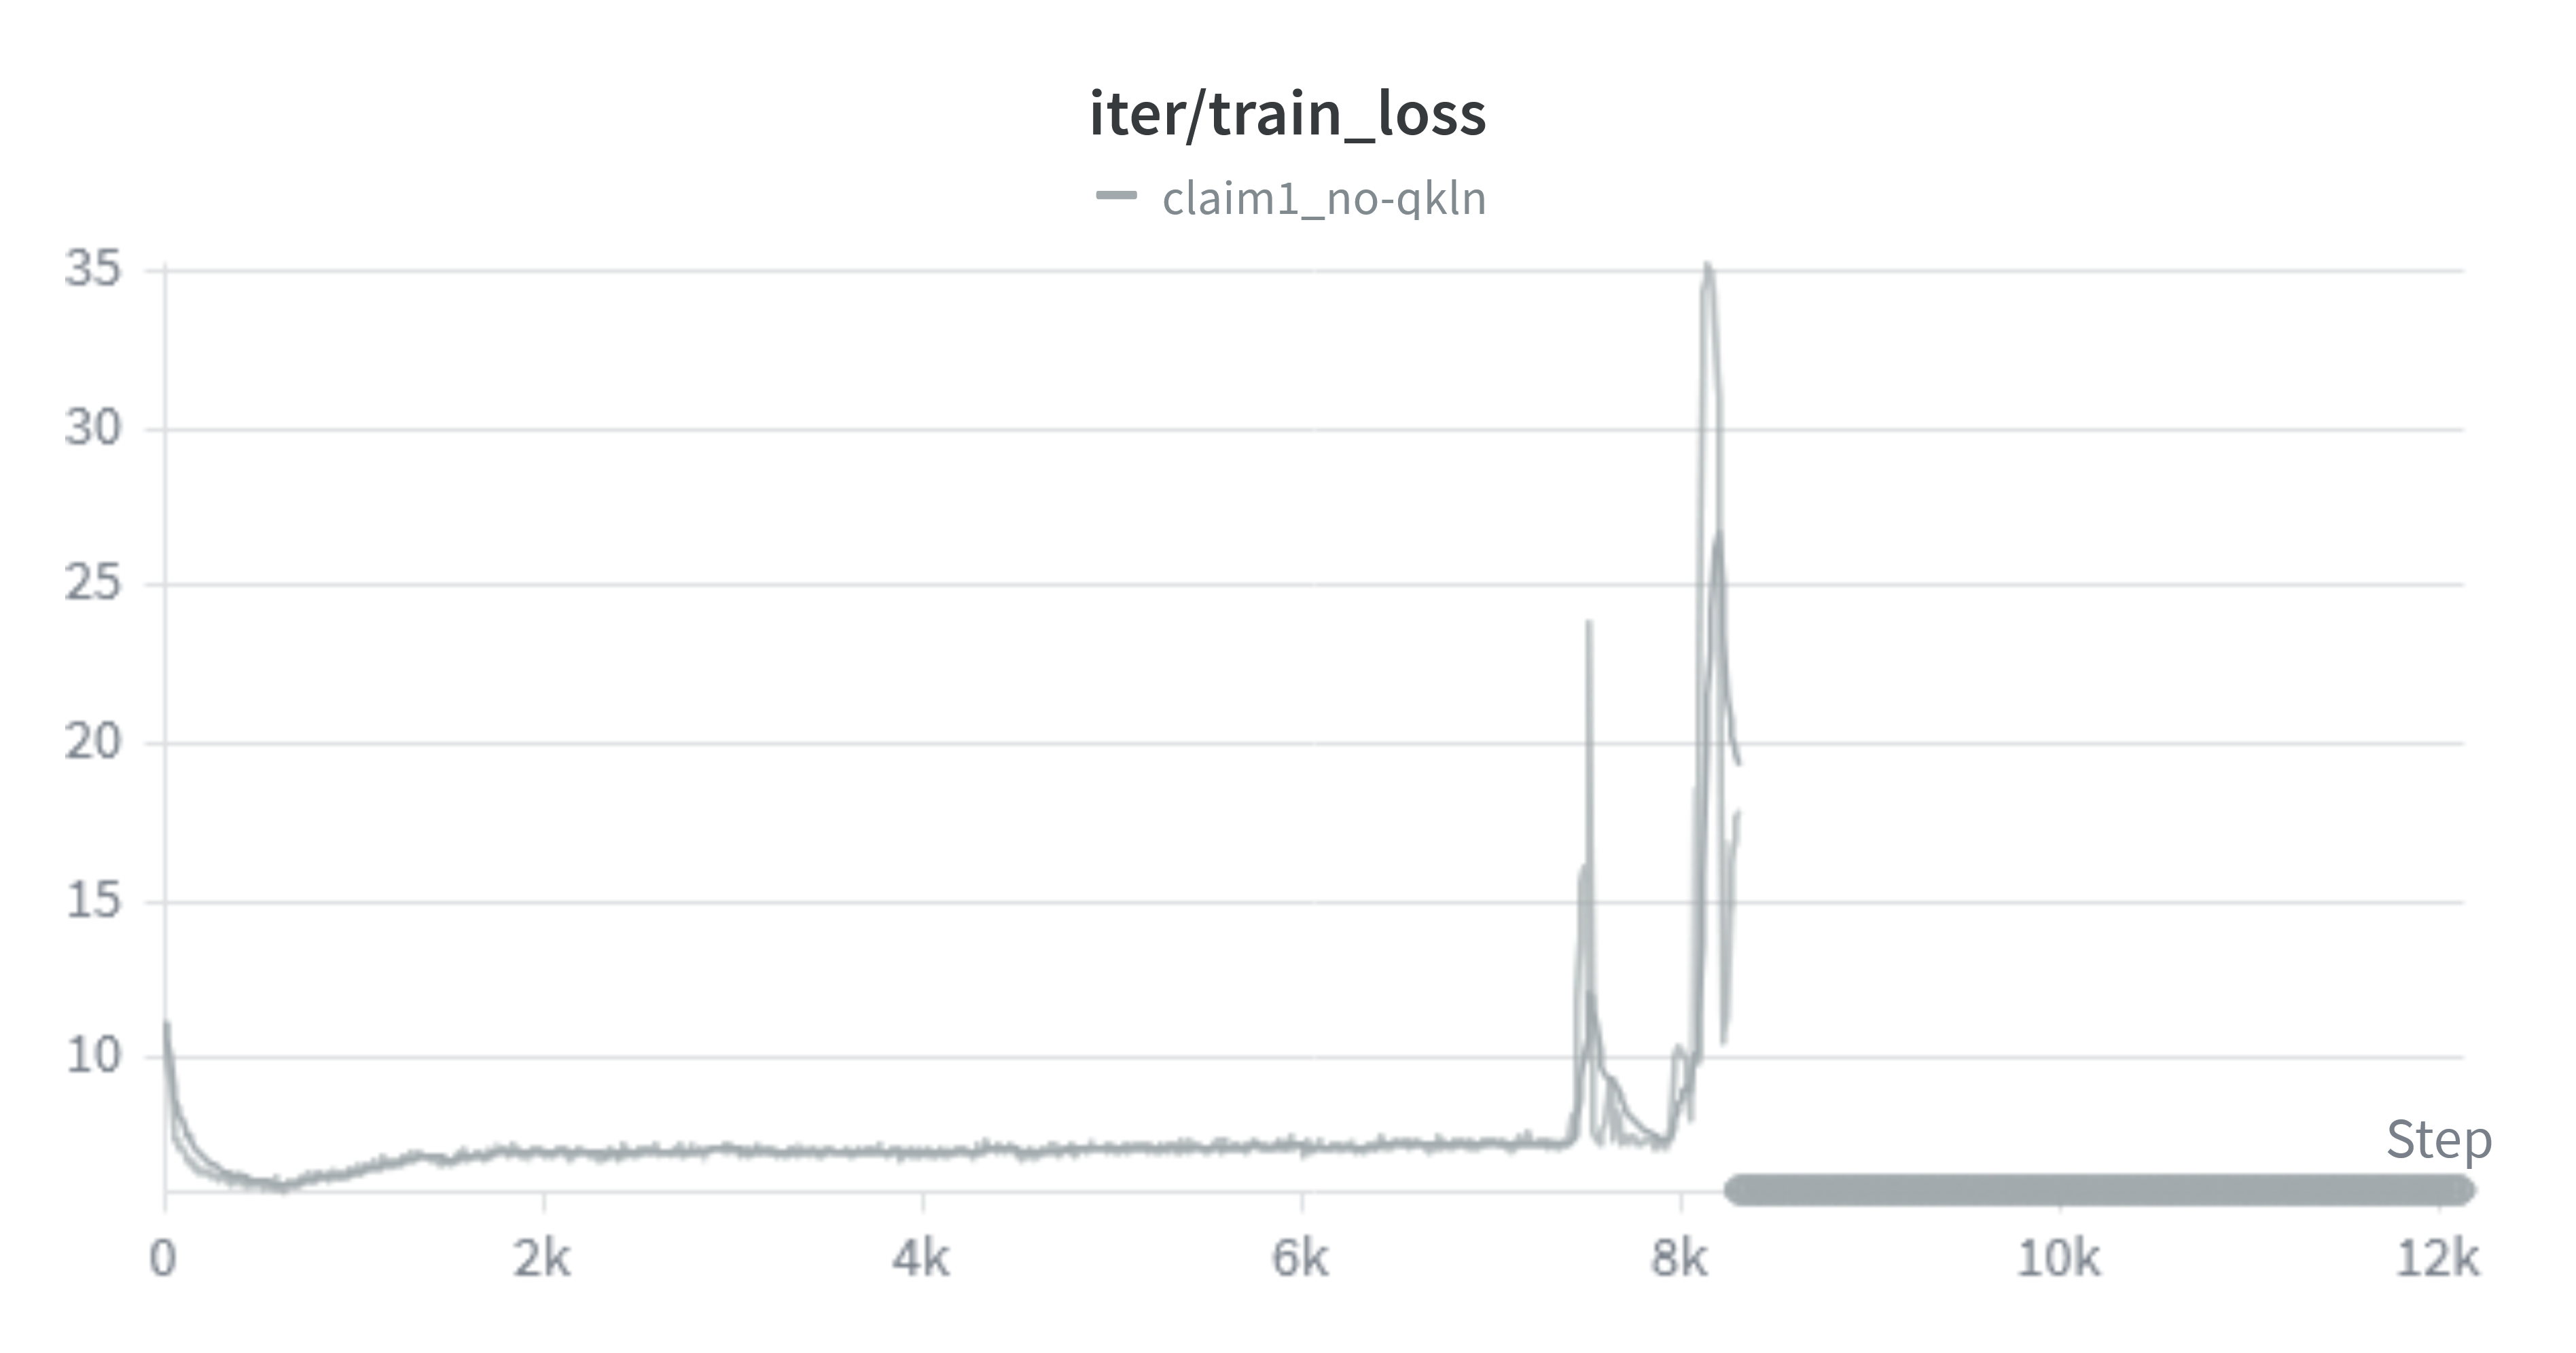
\includegraphics[width=\linewidth]{figures/C2_train_unstable.png}
        \caption{Unstable — train loss}
    \end{subfigure}
    \hfill
    \begin{subfigure}{0.48\textwidth}
        \centering
        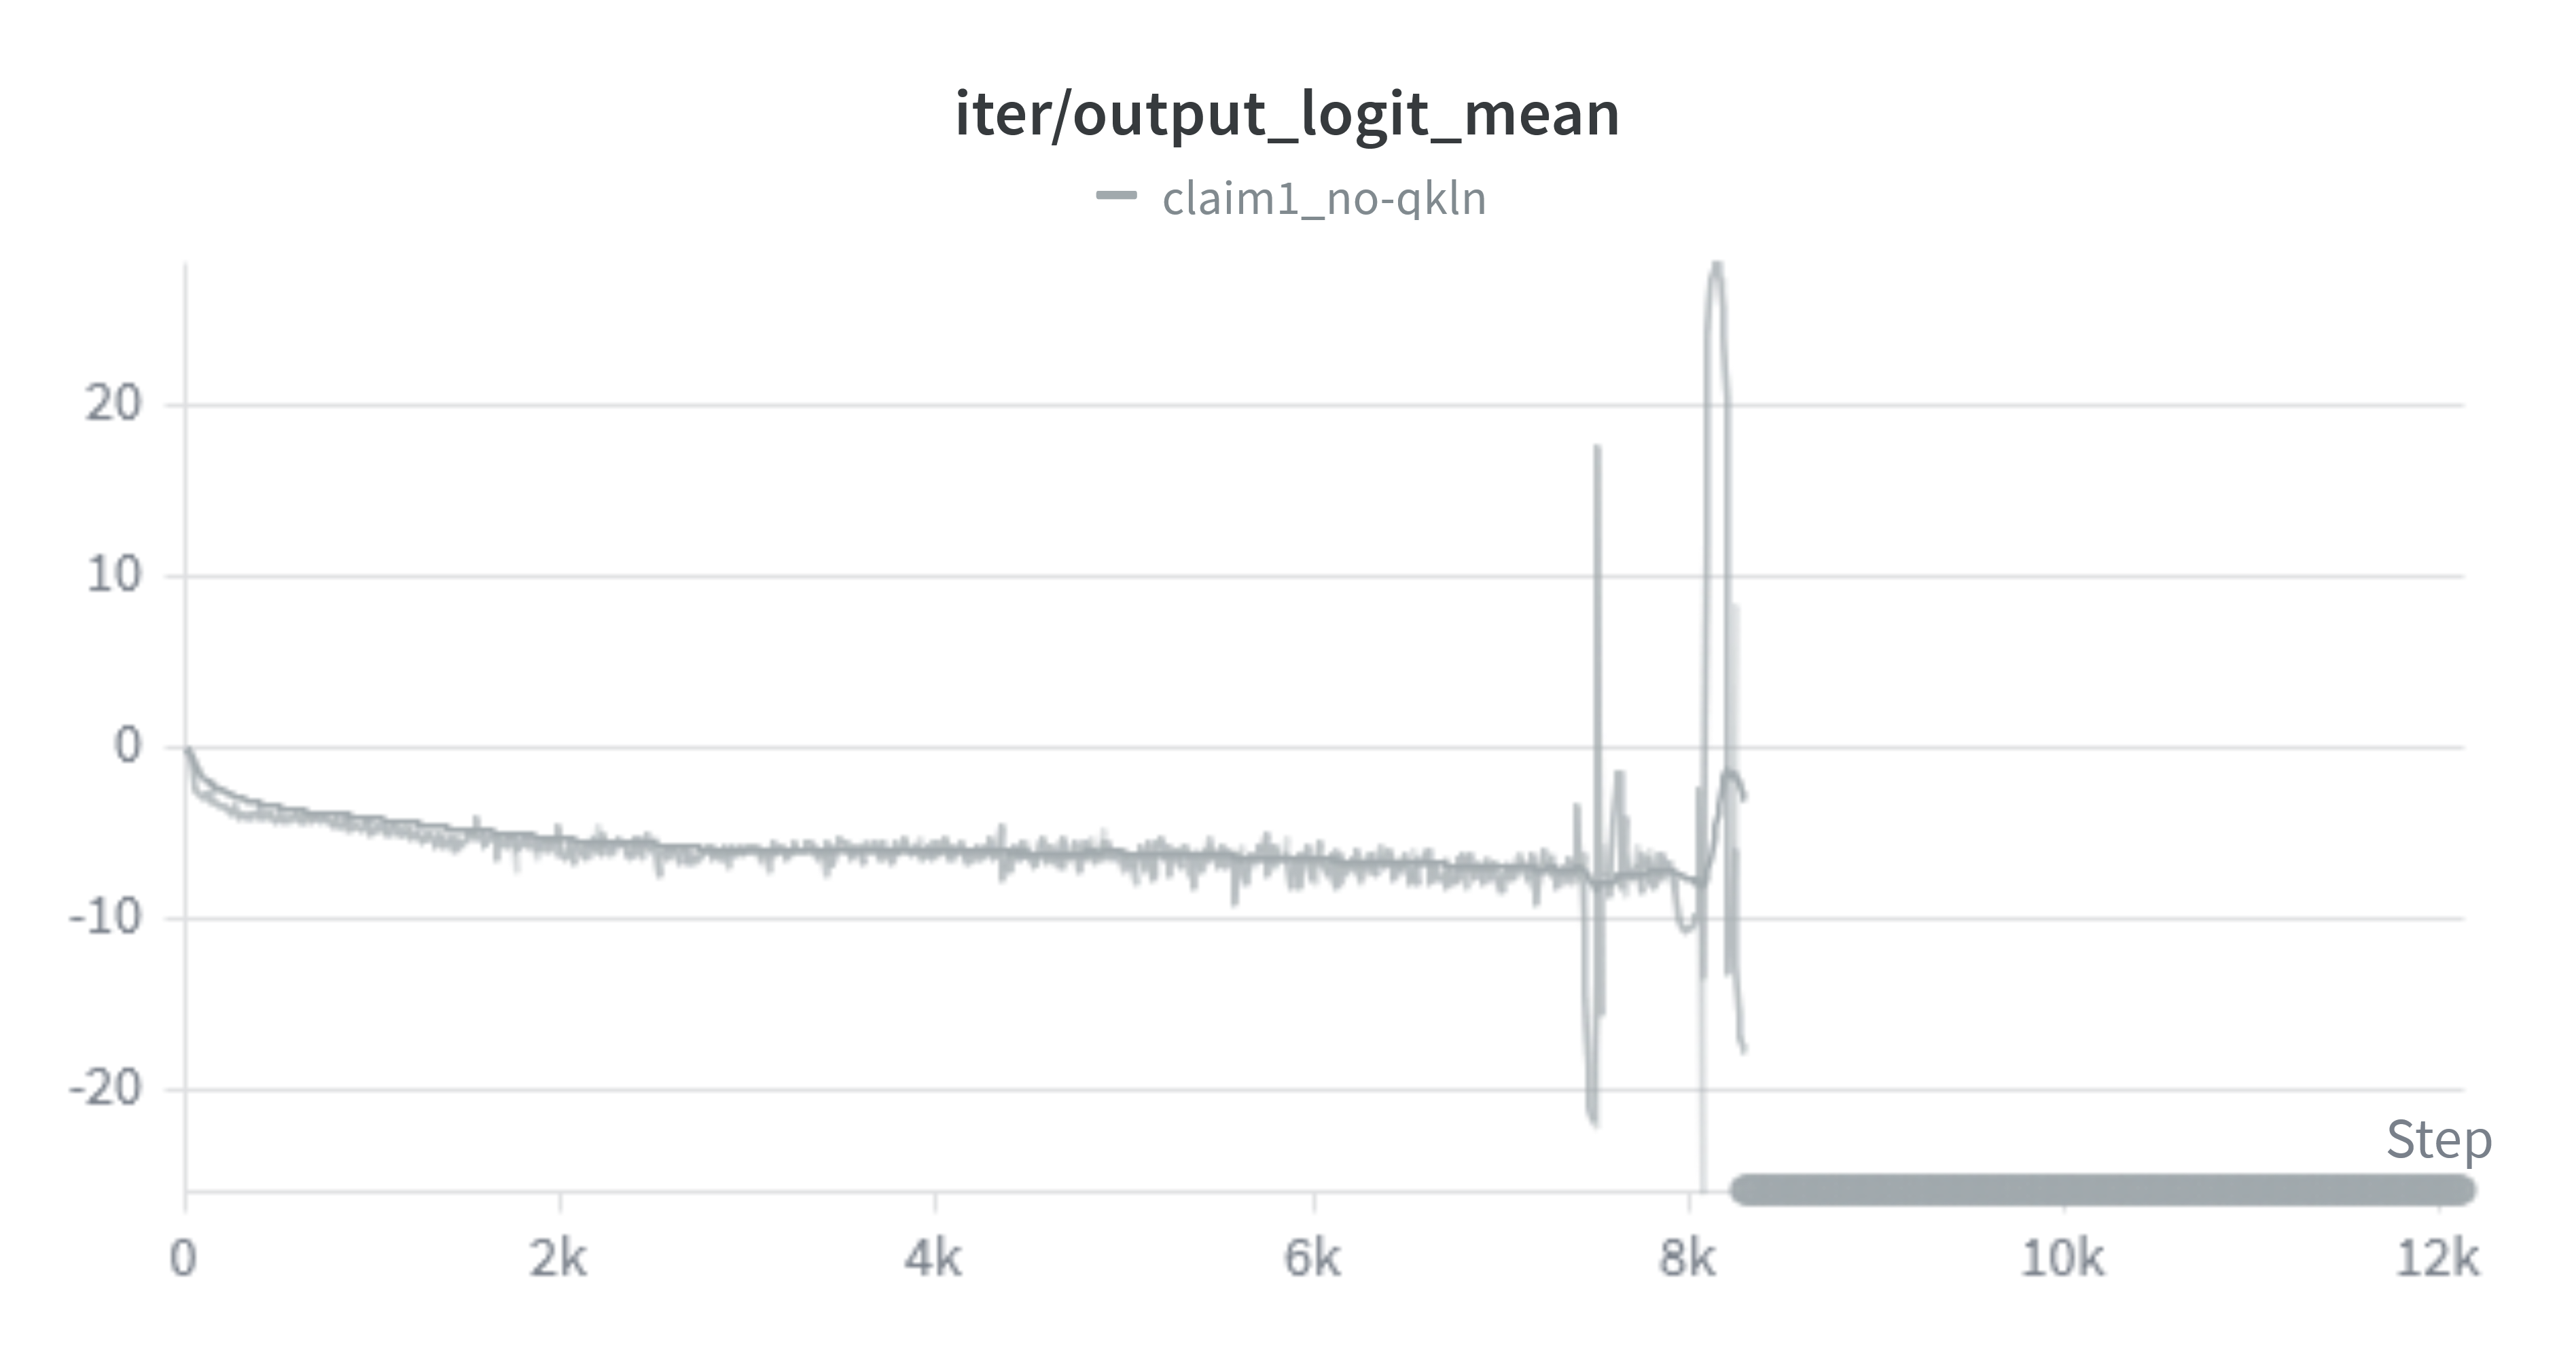
\includegraphics[width=\linewidth]{figures/C2_mean_unstable.png}
        \caption{Unstable — logit mean}
    \end{subfigure}

    \caption{Claim 2 experiments across three regimes. Top: stable training run(lr=0.1). Middle: moderately stable regime with mild fluctuations(lr linear warmup to 0.5). Bottom: unstable regime showing divergence. In three cases we did not observe a collapse to $-\infty$}
    \label{fig:claim2_grid}
\end{figure}
\paragraph{Takeaway.}
Our experiments therefore remain inconclusive for Claim~2.
They suggest that reproducing output-logit divergence may be more sensitive to
implementation details, model scale, or optimisation choices than suggested by
the simplified small-scale protocol alone.
